\documentclass[9pt,ignorenonframetext,mathserif,aspectratio=169,xcolor=dvipsnames]{beamer}
\usetheme{CambridgeUS}

%%%%%%%%%%%%%%
%%    Beamer options   %%
%%%%%%%%%%%%%%

\setbeamertemplate{items}[ball]
\setbeamertemplate{blocks}[rounded][shadow=true]
\setbeamertemplate{navigation symbols}{}
%\usepackage[usenames,dvipsnames]{xcolor}
\hypersetup{colorlinks,urlcolor=blue}
\usepackage[makeroom]{cancel}
\usepackage{media9}
\usepackage{stackengine} % For layering elements
\usepackage{relsize,multirow}
\usepackage{natbib}
\usepackage{hanging}
\usepackage{ragged2e}
\usepackage[export]{adjustbox}   % for left alignment in includegraphics
\setlength{\columnsep}{10pt}

% Calculus symbols
\newcommand{\pd}[2]{\frac{\partial #1}{ \partial #2}}   % First partial derivative command
\newcommand{\td}[2]{\frac{\mathrm{d} #1}{ \mathrm{d} #2}} % First derivative
\newcommand{\md}[2]{\frac{\mathrm{D} #1}{ \mathrm{D} #2}} % Material derivative
\newcommand{\pdd}[2]{\frac{\partial^2 #1}{ \partial #2 ^2}}   % Second partial derivative command
\newcommand{\pddc}[3]{\frac{\partial^2 #1}{ \partial #2 \partial #3}}   % Second partial derivative command
\newcommand{\bs}[1]{\boldsymbol{#1}}
\newcommand{\mbf}[1]{\mathbf{#1}}
\newcommand{\mbfh}[1]{\hat{\mathbf{#1}}}
\newcommand{\etal}{\textit{et al}. }

% Continuum mechanics & FEM symbols
\def\sca   #1{\mbox{\rm{#1}}{}}
\def\mat   #1{\mbox{\boldmath $\mathsf #1$}}
\def\vec   #1{\mbox{\boldmath $#1$}{}}
\def\ten   #1{\mbox{\boldmath $#1$}{}}
\def\Ass  {\overset{\hspace*{0.4cm} n_{\scas{el}}}
	{\underset{\scaf{c},\scaf{d}=1}{\msf{A}}}}


\def\ltr   #1{\mbox{\sf{#1}}}
\def\bltr  #1{\mbox{\sffamily{\bfseries{{#1}}}}}

% math operators and symbols
\DeclareMathOperator{\trace}{trace}
\DeclareMathOperator{\tr}{tr}
\DeclareMathOperator{\symm}{symm}
\DeclareMathOperator{\sk}{skew}
\DeclareMathOperator{\grad}{grad}
\DeclareMathOperator{\Grad}{Grad}
\DeclareMathOperator{\dive}{div}
\DeclareMathOperator{\Dive}{Div}
\DeclareMathOperator{\curl}{curl}
\DeclareMathOperator{\Curl}{Curl}
%\DeclareMathOperator{\Assembly}{\mbox{\mathbb{A}} }
\DeclareMathOperator*{\A}{ \mathlarger{\mathlarger{\boldsymbol{\mathbb{A}}}} }
\newcommand{\vectwo}[2]{\begin{bmatrix} #1 \\ #2 \end{bmatrix}}
\newcommand{\mattwo}[4]{\begin{bmatrix} #1 & #2\\ #3 & #4 \end{bmatrix}}
\newcommand{\vecthree}[3]{\begin{bmatrix} #1 \\ #2 \\ #3 \end{bmatrix}}

\newcommand{\arginf}{\mathop{\mathrm{arg\,inf}}}
\newcommand{\argsup}{\mathop{\mathrm{arg\,sup}}}
\def\d#1{\mbox{$\,\mathrm{d}#1$}}
\def\order#1{\mbox{$\mathcal{O}(#1)$}}
\def\python{\mbox{\tt Python}}
\def\R{\mbox{\(\mathbb{R}\)}}
\def\dx{\mbox{\(\,\mathrm{d}x\)}}
\def\TODO{\mbox{\tt TODO}}


%%%  Theorem declaration  %%%
\newtheorem{thm}{\hspace{0.5cm}}
\newtheorem{lema}{\bf{Lema}}
%\newtheorem{example}{\bf{Ejemplo}}
\newtheorem{defn}{\bf{Definici\'{o}n}}
\newtheorem{prop}{\bf{Proposici\'{o}n}}
%\newtheorem{corollary}{\bf{Corolario}}
%\newtheorem{proof}{\bf{Demostraci\'{o}n}}
\newtheorem{soln}{\bf{Soluci\'{o}n}}
\newtheorem{rmk}{\bf{Nota}}
\newtheorem{objgen}{\bf{Objetivo}}

\newcommand{\backupbegin}{
   \newcounter{finalframe}
   \setcounter{finalframe}{\value{framenumber}}
}
\newcommand{\backupend}{
   \setcounter{framenumber}{\value{finalframe}}
}
\usepackage{moreverb}
\usepackage{amsmath, amsfonts, amsthm,alltt}
\usepackage{multirow, hyperref}

\usepackage[absolute,showboxes,verbose,overlay]{textpos}
\usepackage[font={footnotesize}]{caption}
\captionsetup{justification=centering,singlelinecheck=false, labelformat=empty }


% Paquete para escribir codigo
\usepackage{listings}
\usepackage{graphicx}
\usepackage{blkarray}
%\usepackage{color}
%\usepackage[usenames,dvipsnames]{xcolor}

\lstset{basicstyle=\footnotesize\ttfamily,breaklines=true}

\setbeamertemplate{itemize/enumerate body begin}{\large}
\setbeamertemplate{itemize/enumerate subbody begin}{\normalsize}

% page numbering
%\setbeamertemplate{footline}{\begin{center} \small \insertframenumber \end{center}}
%\setbeamertemplate{headerline}{\begin{center} \small \insertframenumber \end{center}}
%\setbeamertemplate{footline}{\hfill\small\insertframenumber/\inserttotalframenumber}1

%\usepackage{beamerarticle} // not installed
%\usepackage{beamerthemesplit} // Activate for custom appearance

\makeatother
\setbeamertemplate{footline}
{\hfill\insertframenumber/ \inserttotalframenumber\hspace*{1ex}}
\date{\center \tiny \textit{École Normale Supérieure}, Paris \\ August 2026 }
%%%%%%%%
% Author data %
%%%%%%%%
	\vspace{2cm}
	\title{From Physics-Based Earthquake Catalogs to Seismic Hazard: \\ First Steps with VEGA}
\author{ Pablo Iturrieta\inst{1}}
\institute{\raggedright \inst{1} GFZ German Research Centre for Geosciences}

%%%%%%%%
% Document %
%%%%%%%%

\begin{document}

\begin{frame}[t]
\mbox{}%
	\begin{minipage}{0.22\textwidth}
		\centering
	
\includegraphics[width=1\textwidth]{./figures/logo_gfz}
	\end{minipage}%

\maketitle
\end{frame}

-----------------------------------------------------

\begin{frame}[t]
\frametitle{What is Probabilistic Seismic Hazard Analysis (PSHA)?}

  Estimates the probability that ground motion at a site exceeds a given
  intensity level.\\

\only<2-4>{
\begin{columns}[T,onlytextwidth]
  \begin{column}{0.65\textwidth}
    \RaggedRight
    \only<3-4>{{\vspace{0.2cm}\begin{center} 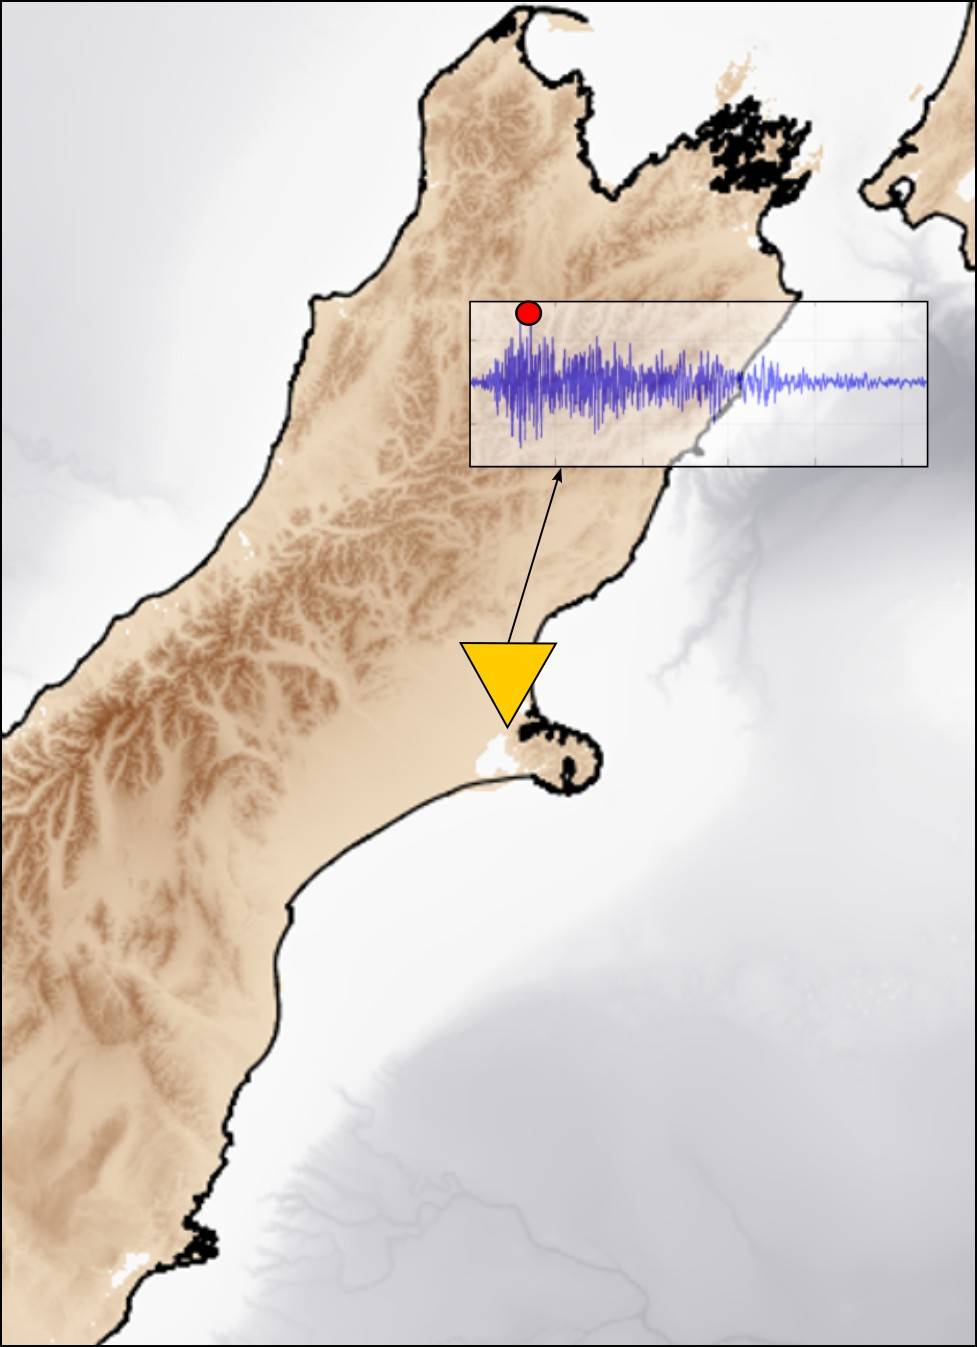
\includegraphics[width=0.4\linewidth]{figures/nz_seism}\end{center}}}
  \end{column}
  \begin{column}{0.35\textwidth}
      \vspace{0.2cm}
    \RaggedLeft
    \only<2>{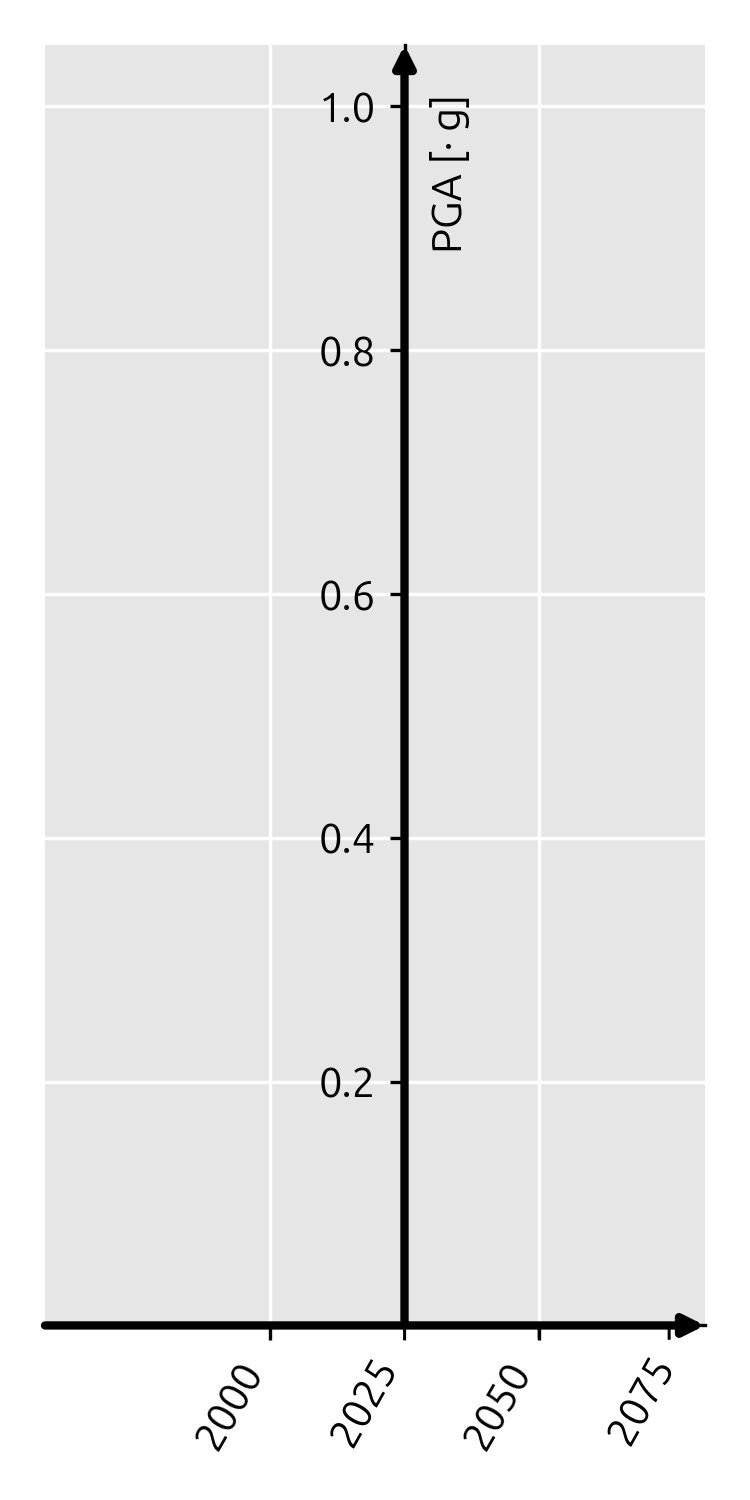
\includegraphics[valign=t,right,max width=0.5\linewidth]{figures/axis1}}
    \only<3>{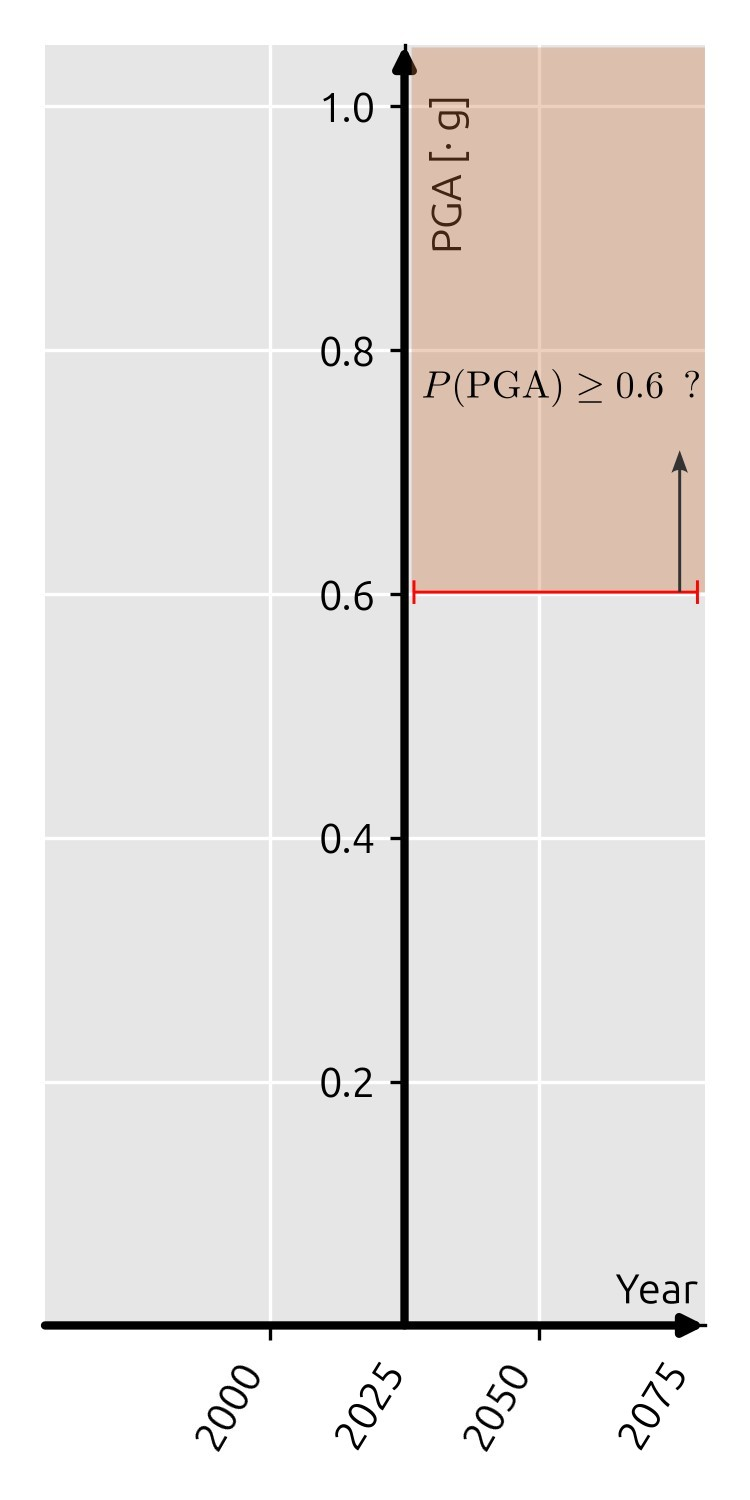
\includegraphics[valign=t,right,max width=0.5\linewidth]{figures/axis}}
    \only<4>{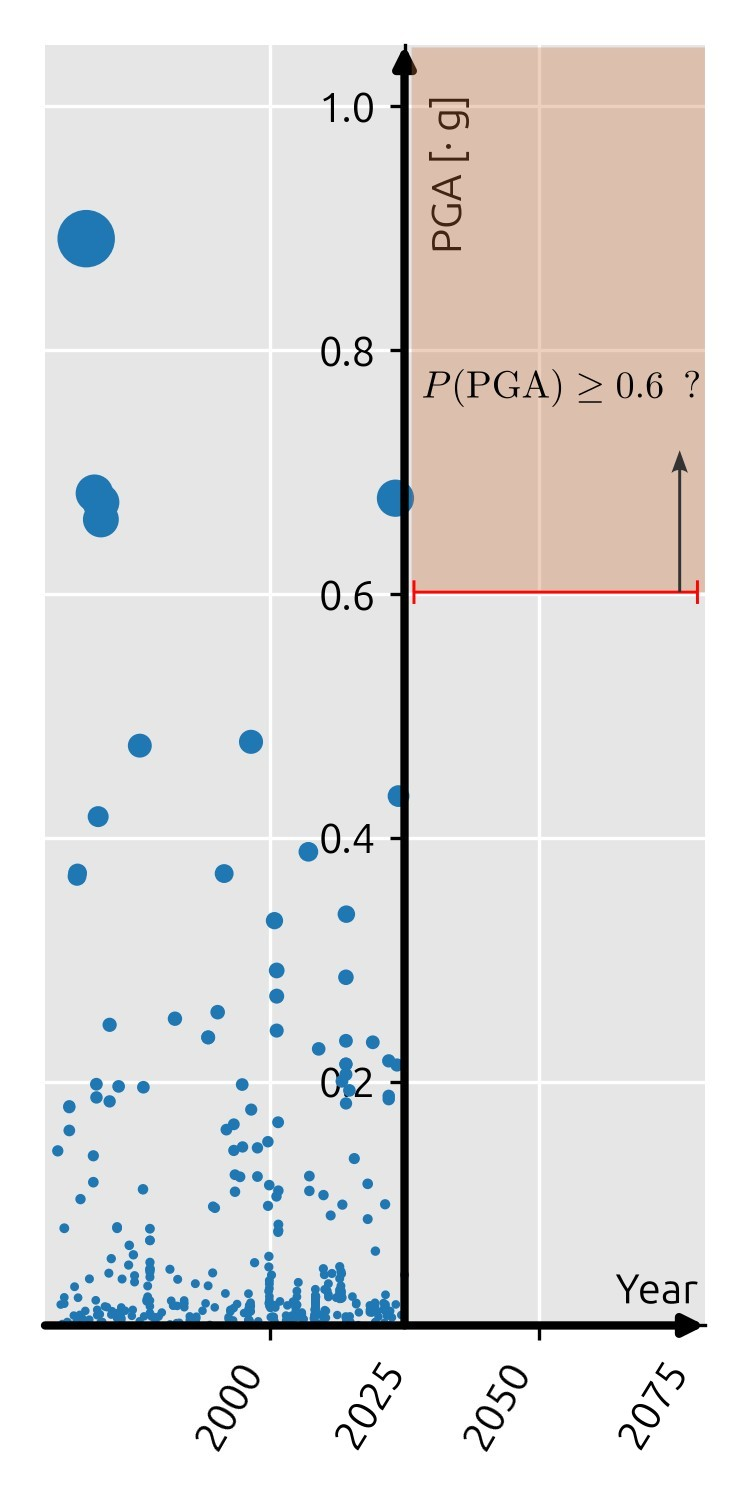
\includegraphics[valign=t,right,max width=0.5\linewidth]{figures/axis2}\hspace{0.1cm}}
  \end{column}
\end{columns}
}

\only<5>{
\begin{columns}[T,onlytextwidth]
  \begin{column}{0.65\textwidth}
    \RaggedRight
    \vspace{0.2cm}
    \begin{center}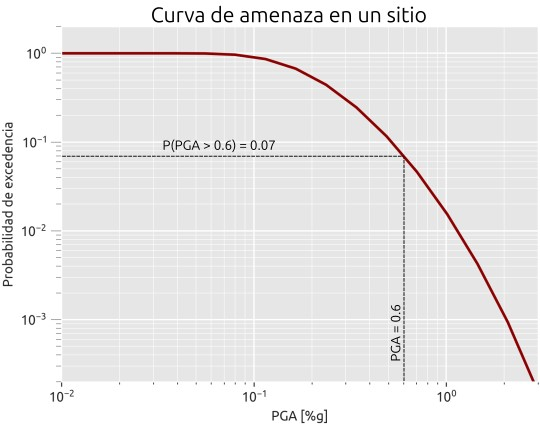
\includegraphics[width=0.8\linewidth]{figures/curva_ejemplo}\end{center}
  \end{column}
  \begin{column}{0.35\textwidth}
      \vspace{0.2cm}
    \RaggedLeft
    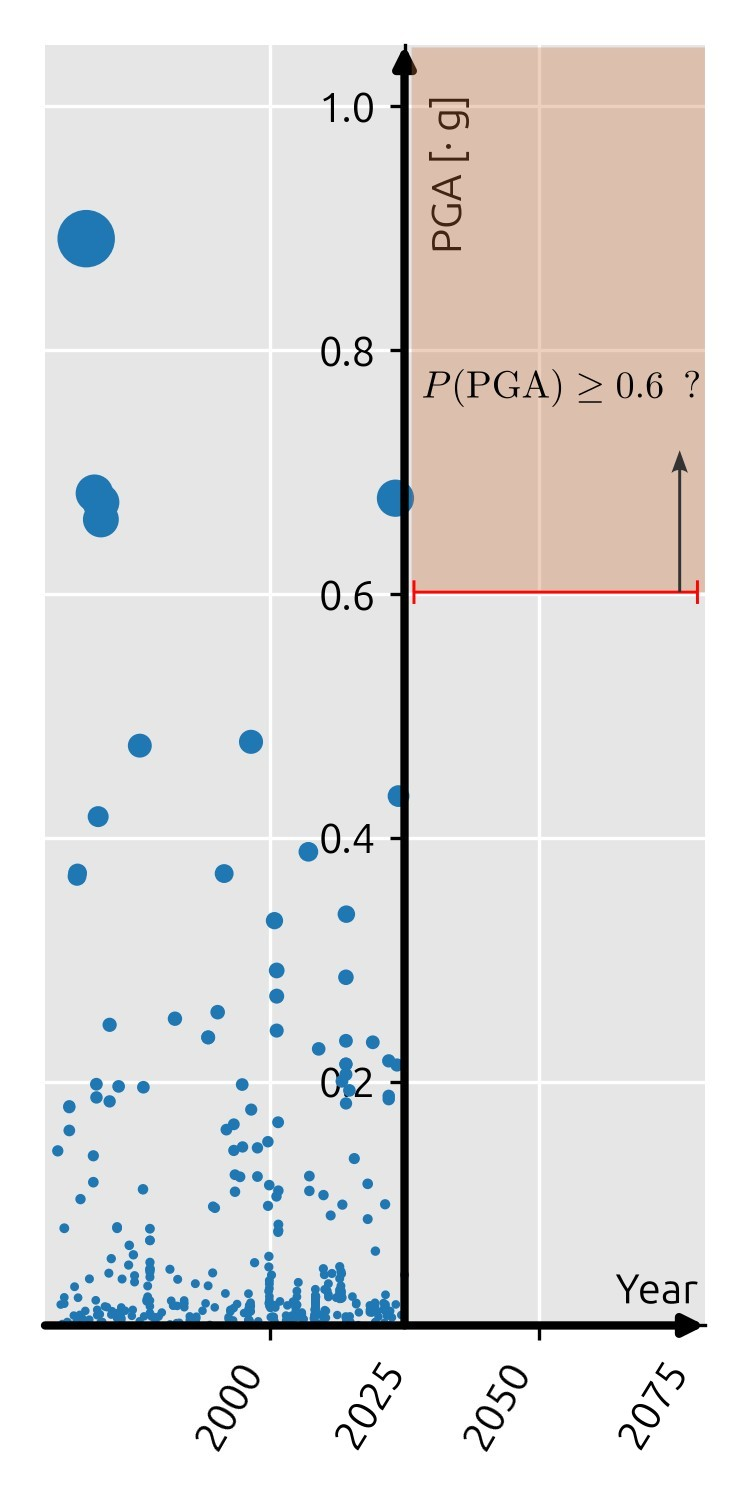
\includegraphics[valign=t,right,max width=0.5\linewidth]{figures/axis2}
  \end{column}
\end{columns}
}
\end{frame}

\begin{frame}[t]
	\frametitle{How a PSHA model is built}

\begin{columns}[t]
	\column{.55\textwidth}
	\vspace{-0.5cm}
	\only<1-4>{
\begin{itemize}
	\item Combines an \textbf{earthquake occurrence} model with a
	      \textbf{ground motion} model.
 \end{itemize}
	}
	\only<2-4>{
	\begin{exampleblock}{\large Earthquake forecasting (probabilistic)}
\begin{itemize}
	\item Identify seismogenic sources.
	\item Space--time distribution of seismicity.
	\item Frequency--magnitude distribution.
\end{itemize}
	\end{exampleblock}
	}
	\only<3-4>{
\begin{alertblock}{\large Ground motion model (GMM)}
	\begin{itemize}
\item Shaking intensity at a site as a function of earthquake
      properties and site conditions.
\end{itemize}
	\end{alertblock}
	}
	\column{.45\textwidth}
	\only<2>{
		\begin{figure}
		\vspace*{-1.5cm}
		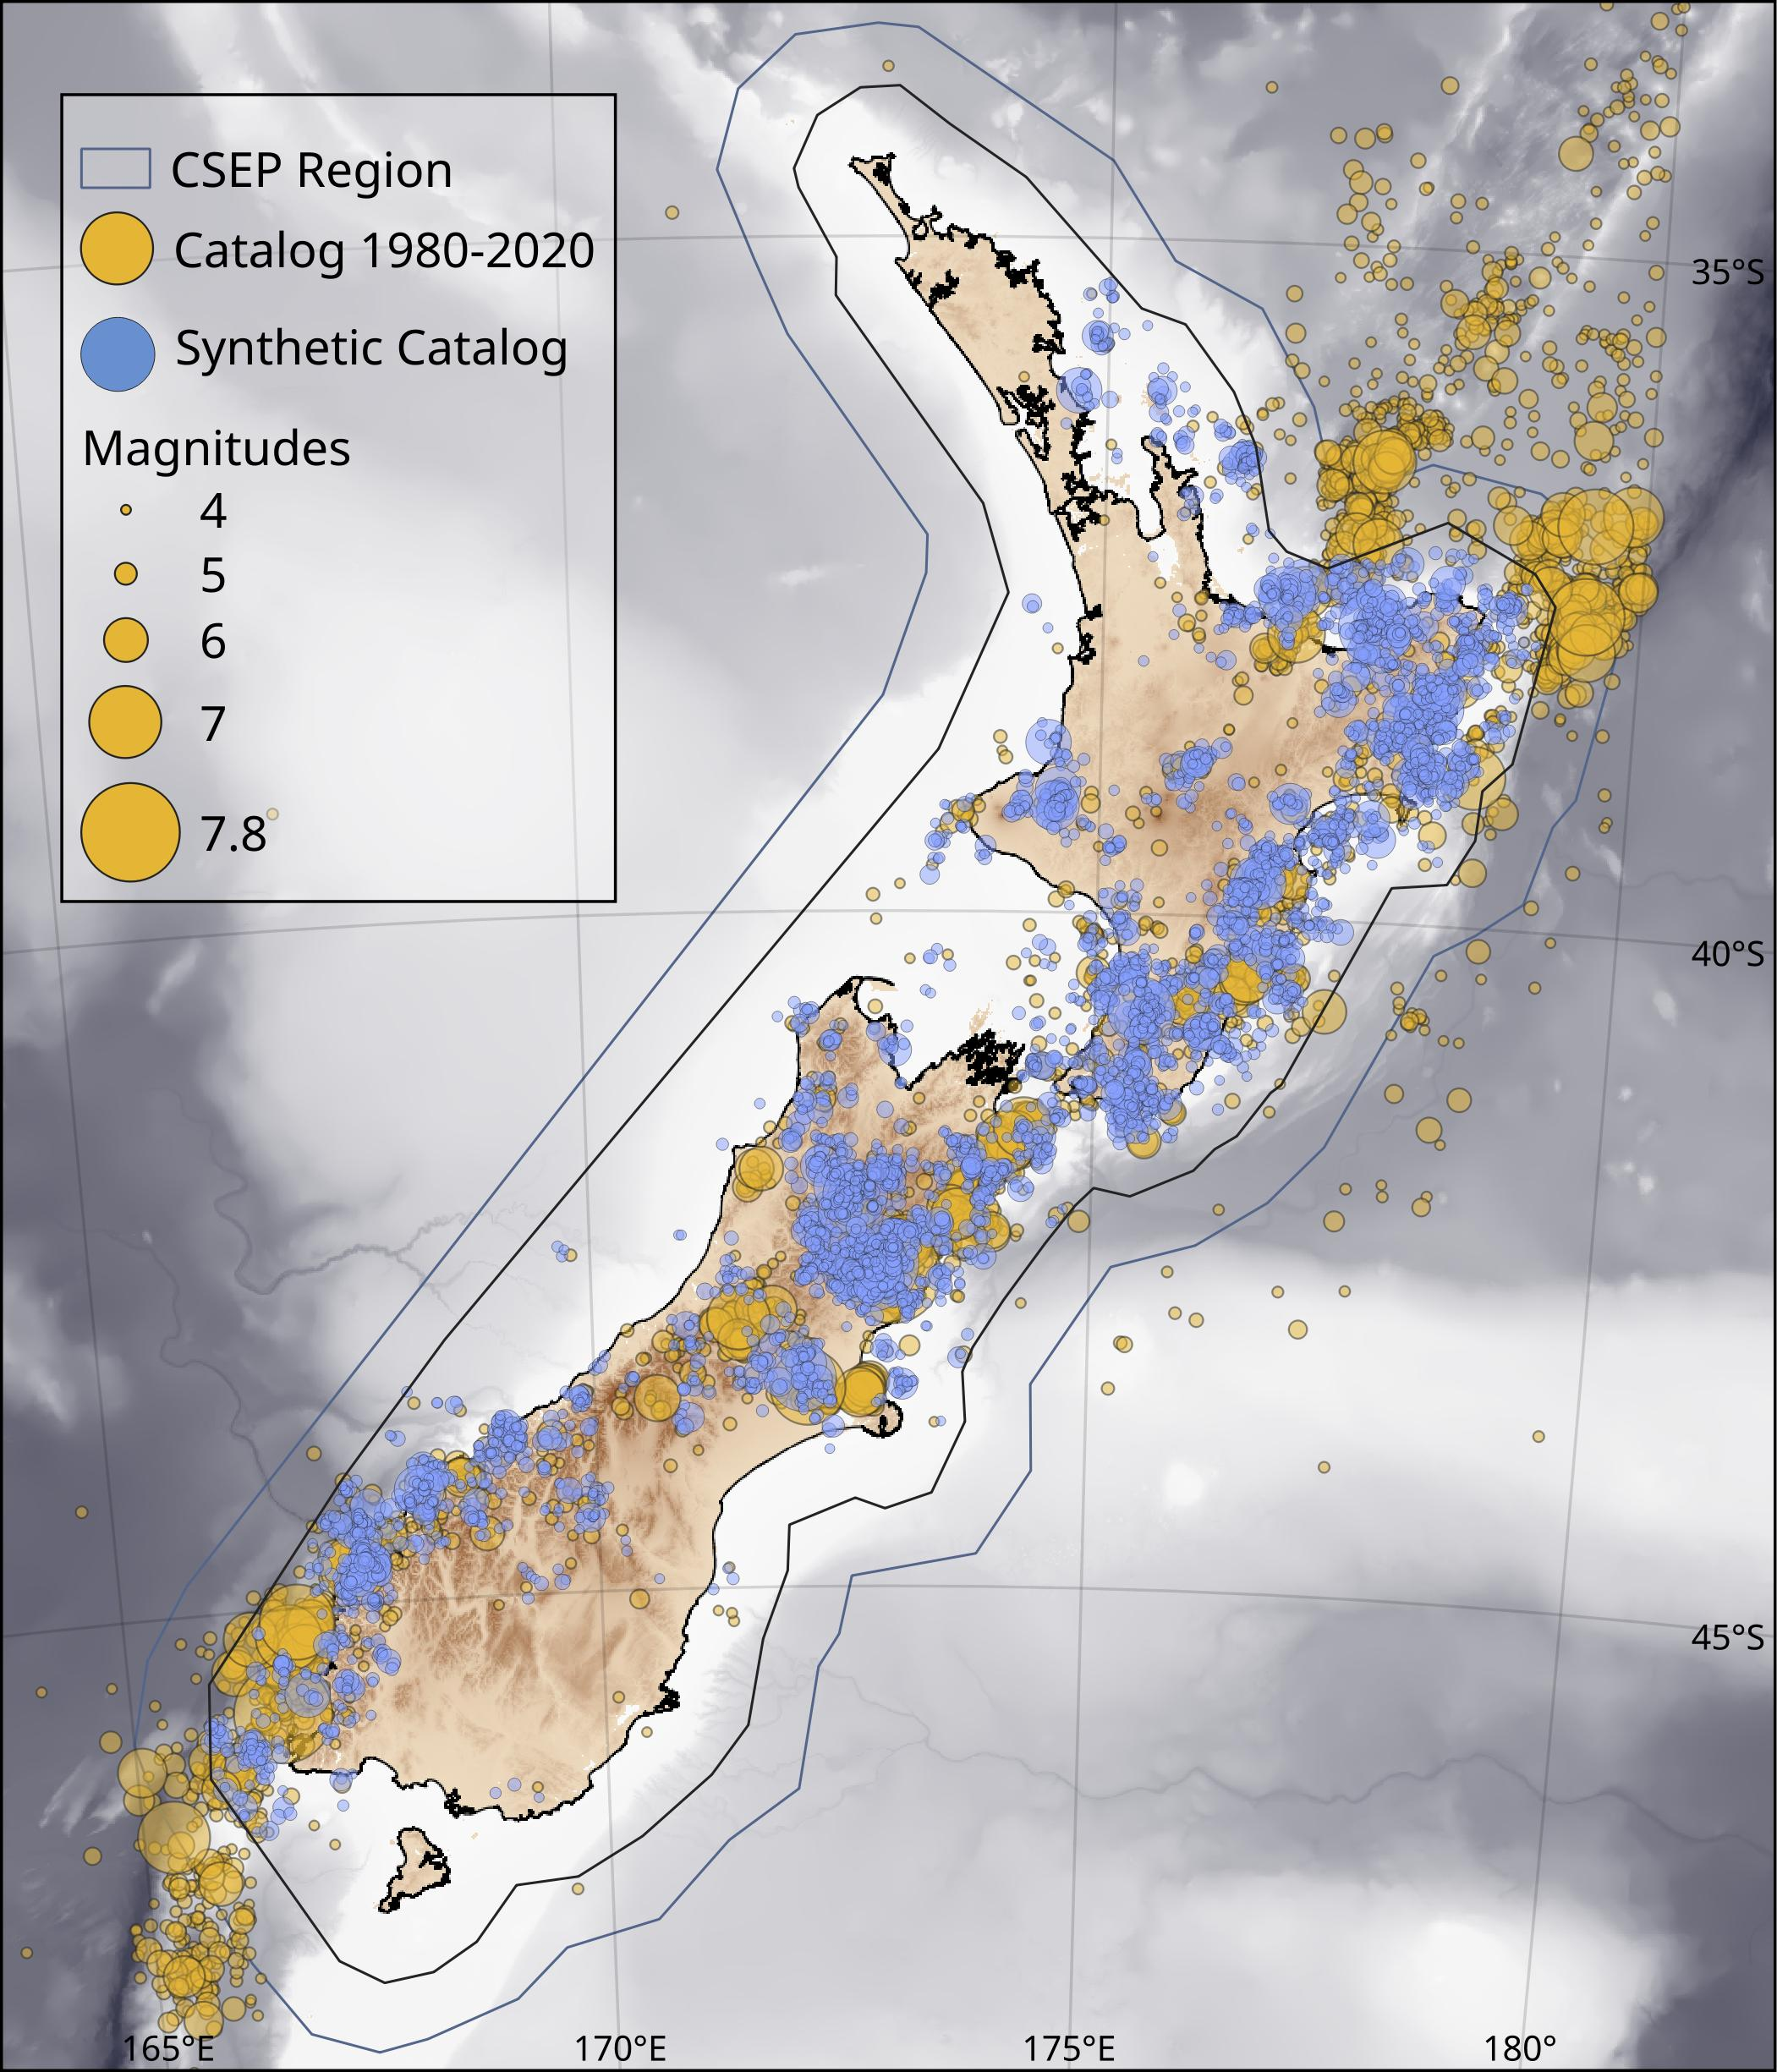
\includegraphics[width=0.9\textwidth]{./figures/catalog_forecast}
		\caption*{\scriptsize One realization of a \textbf{stochastic catalog} model (ETAS) for
		New Zealand crustal seismicity (Iturrieta et al., 2024). Occurrence
		is statistical, not physical.}
	\end{figure}
	}
	\only<3-4>{
	\begin{figure}
		\vspace*{-1.cm}
		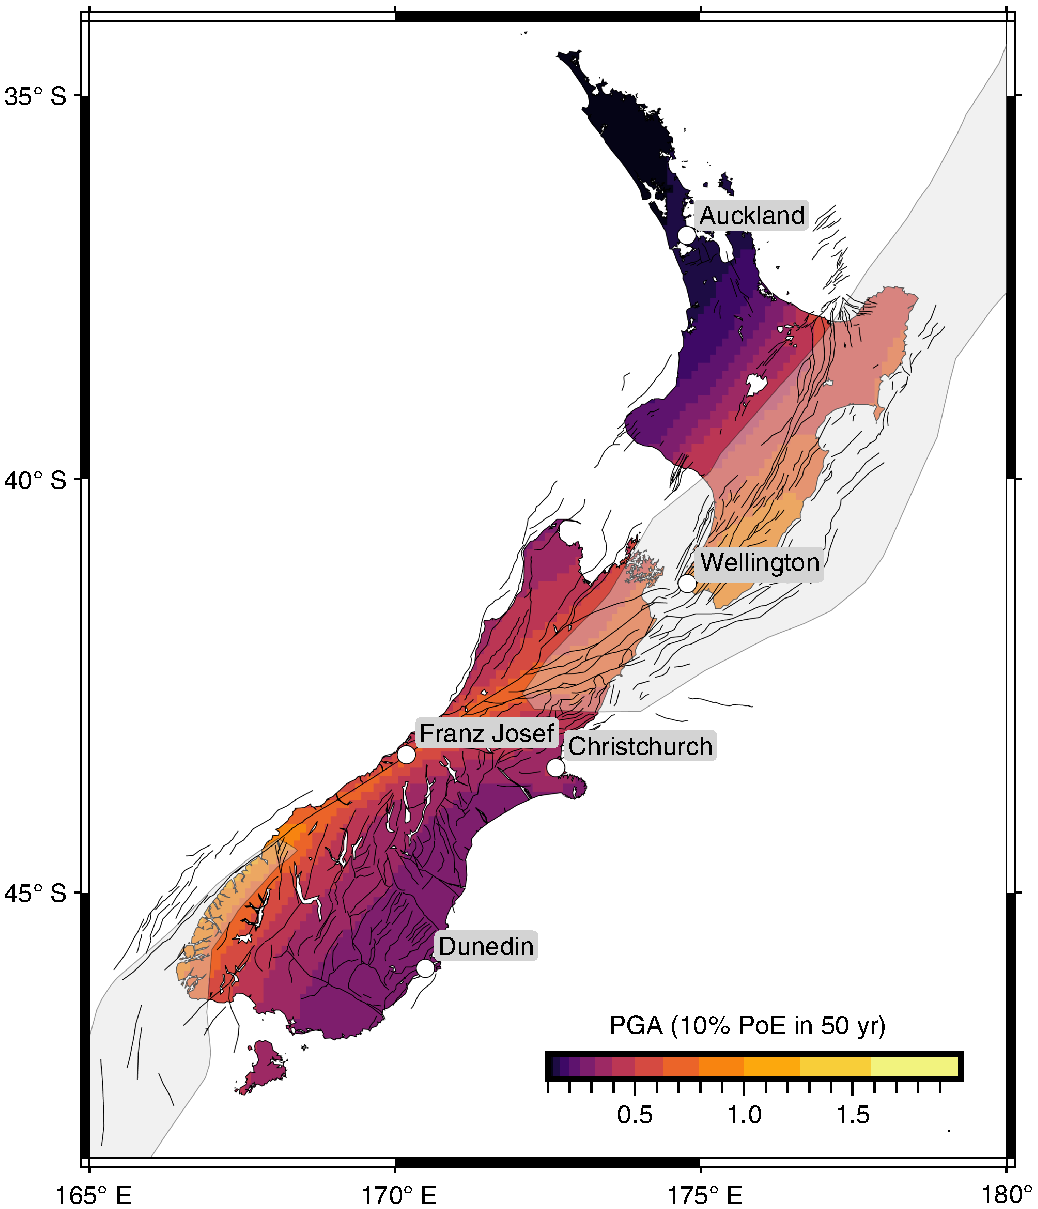
\includegraphics[width=0.85\textwidth]{./figures/hazard_model_nz}
		\caption*{\scriptsize New Zealand seismic hazard model, 2022 (Gerstenberger et al., 2023).
		PGA with 10\% probability of exceedance in 50 years
		($V_{\mathrm{S}30}=250 \, \mathrm{m}/\mathrm{s}$).}
	\end{figure}
	}
\end{columns}
\end{frame}

\begin{frame}[t]
	\frametitle{How crustal faults enter a hazard model today}

	\begin{columns}[t]
		\column{.4\textwidth}
	\begin{itemize}
		\item Gutenberg--Richter or characteristic FMD, \emph{imposed} on each fault.
		\item $M_{max}$ from fault geometry or scaling relations.
		\item Solve for the rate $a$ from a long-term moment budget.
	\end{itemize}
\begin{align*}
	\dot{M}^{\text{long-term}} &= 	\dot{M}^{\mathrm{seismic}} \\
	\dot{M}^{\text{long-term}} &=
\phi\,\mu\,L\,W\,\dot{s}_r
\end{align*}

	Where $\dot{s}_r$ is the slip rate and $\phi$ the seismic/aseismic
	coupling factor.
		\column{.6\textwidth}
		\begin{figure}
		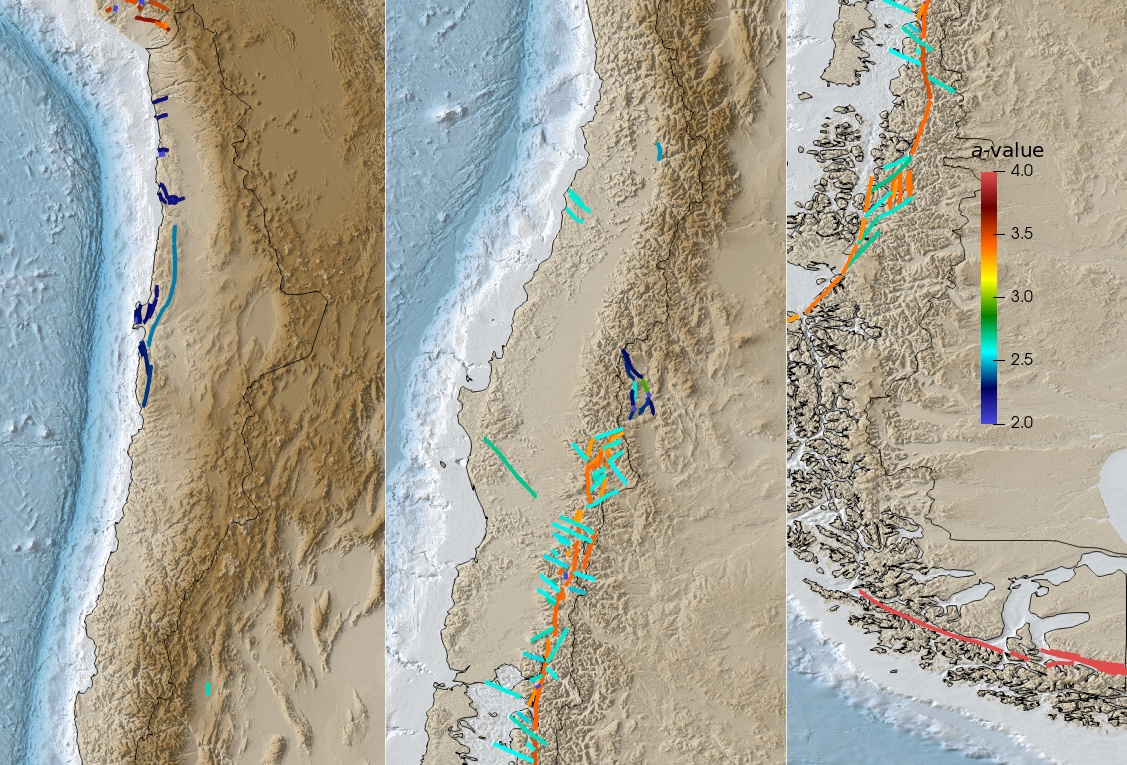
\includegraphics[width=0.95\textwidth]{./figures/a_val_faults}
		\caption*{\scriptsize Fault activity rates for the Chilean model, derived from slip rates.}
		\end{figure}
	\end{columns}
\end{frame}

\begin{frame}[t]
	\frametitle{Seismic hazard map for Chile: faults do matter}

			\begin{figure}
			\vspace*{-0.3cm}
			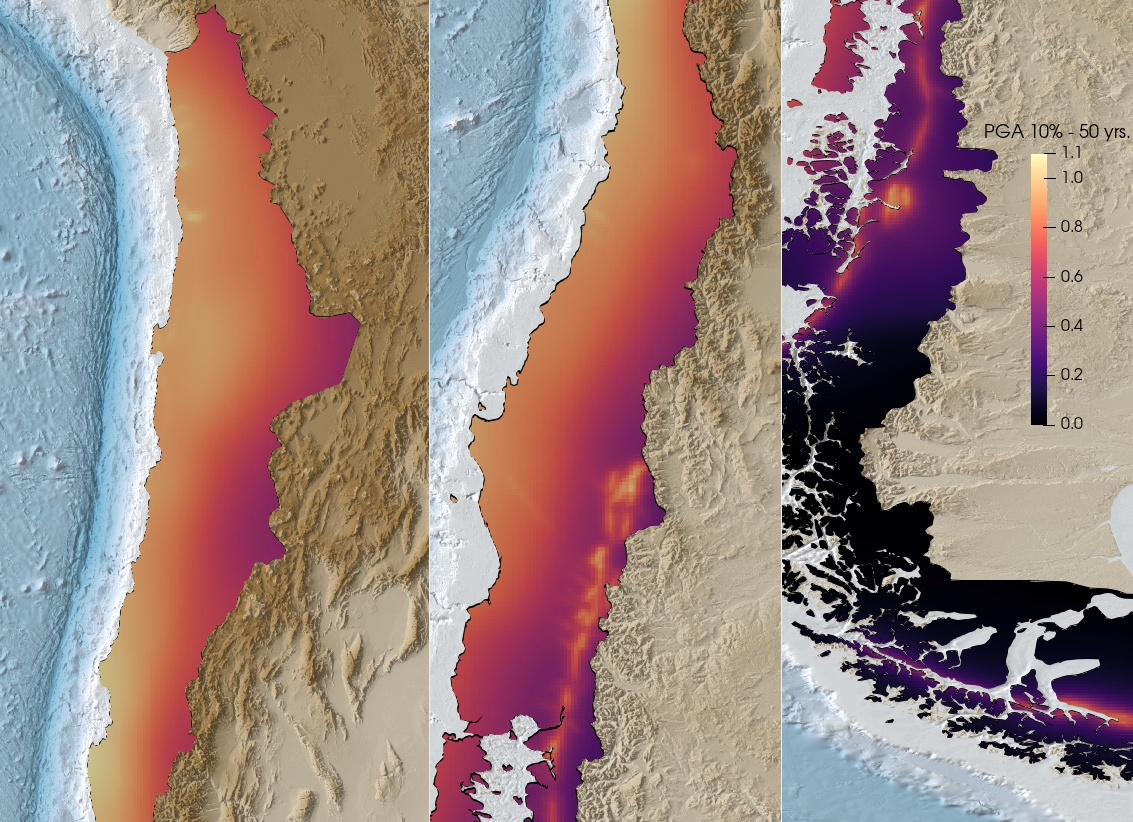
\includegraphics[width=0.6\textwidth]{./figures/hazardmap_faults}
				\caption*{\scriptsize Hazard map \textbf{including} crustal faults, subduction and intraplate earthquakes: PGA with 10\%
				probability of exceedance in 50 years,
				$V_{\mathrm{S}30}=250 \, \mathrm{m}/\mathrm{s}$.
				Computed with OpenQuake (Pagani et al., 2012).}
			\end{figure}

\end{frame}

%% ------------------------------------------------------------------
%% PART 2 - The assumptions we would like to relax
%% ------------------------------------------------------------------

\begin{frame}[t]\frametitle{The assumptions we would like to relax}

Everything in the previous slide rests on a set of convenient
assumptions:

\begin{itemize}
  \item<1-> \textbf{Poisson occurrence}: earthquakes are independent and
        memoryless. No seismic cycle, no clustering, no triggering.
  \item<2-> \textbf{Imposed magnitude distribution}: a Gutenberg--Richter
        law is prescribed per source, rather than emerging from the
        mechanics.
  \item<3-> \textbf{Independent sources}: faults do not talk to each other.
        No static stress transfer, no multi-fault ruptures.
\end{itemize}

\vspace{0.3cm}
\only<5>{
\begin{exampleblock}{\large The question of this work}
Can a \textbf{physics-based} earthquake simulator produce synthetic
catalogs from which hazard is computed \emph{without} any of these
assumptions, and how different are the results?
\end{exampleblock}
}
\end{frame}

%% ------------------------------------------------------------------
%% PART 3 - The synthetic catalog
%% ------------------------------------------------------------------

\begin{frame}[t]
	\frametitle{Synthetic catalogs with VEGA}

	\begin{columns}[t]
		\column{.42\textwidth}
		\textbf{What we prescribe:}
		\begin{itemize}\small
			\item A fault network: one main fault ($L \approx 25$ km),
			      quasi-parallel structures, and a damage zone of
			      off-fault sources.
			\item Rate-and-state friction
			\item A background stress state and a constant shear
			      loading rate.
		\end{itemize}

		\vspace{0.2cm}
		\textbf{What we do \emph{not} prescribe:}
		\begin{itemize}\small
			\item When earthquakes happen.
			\item How big they are.
			\item Whether they cluster, cascade, or repeat.
		\end{itemize}
		\column{.58\textwidth}
		\begin{figure}
		\vspace*{-0.7cm}
		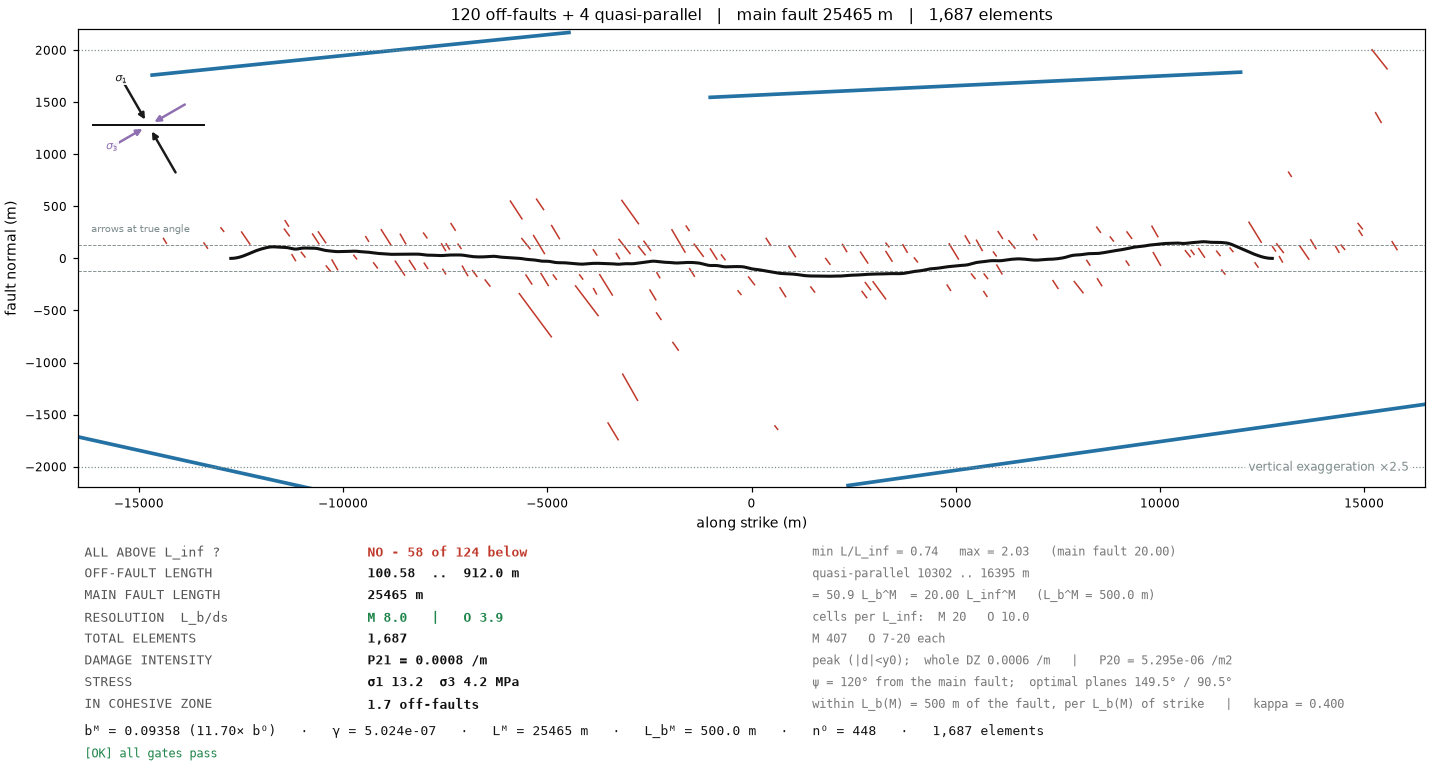
\includegraphics[width=1\textwidth]{./figures/fault_v6}
		\caption*{\scriptsize Fault network generated for the experiment.}
		\end{figure}
	\end{columns}
\end{frame}

\begin{frame}[t]
	\frametitle{The resulting catalog}

	\only<1>{
		\begin{figure}
		\vspace*{-0.3cm}
		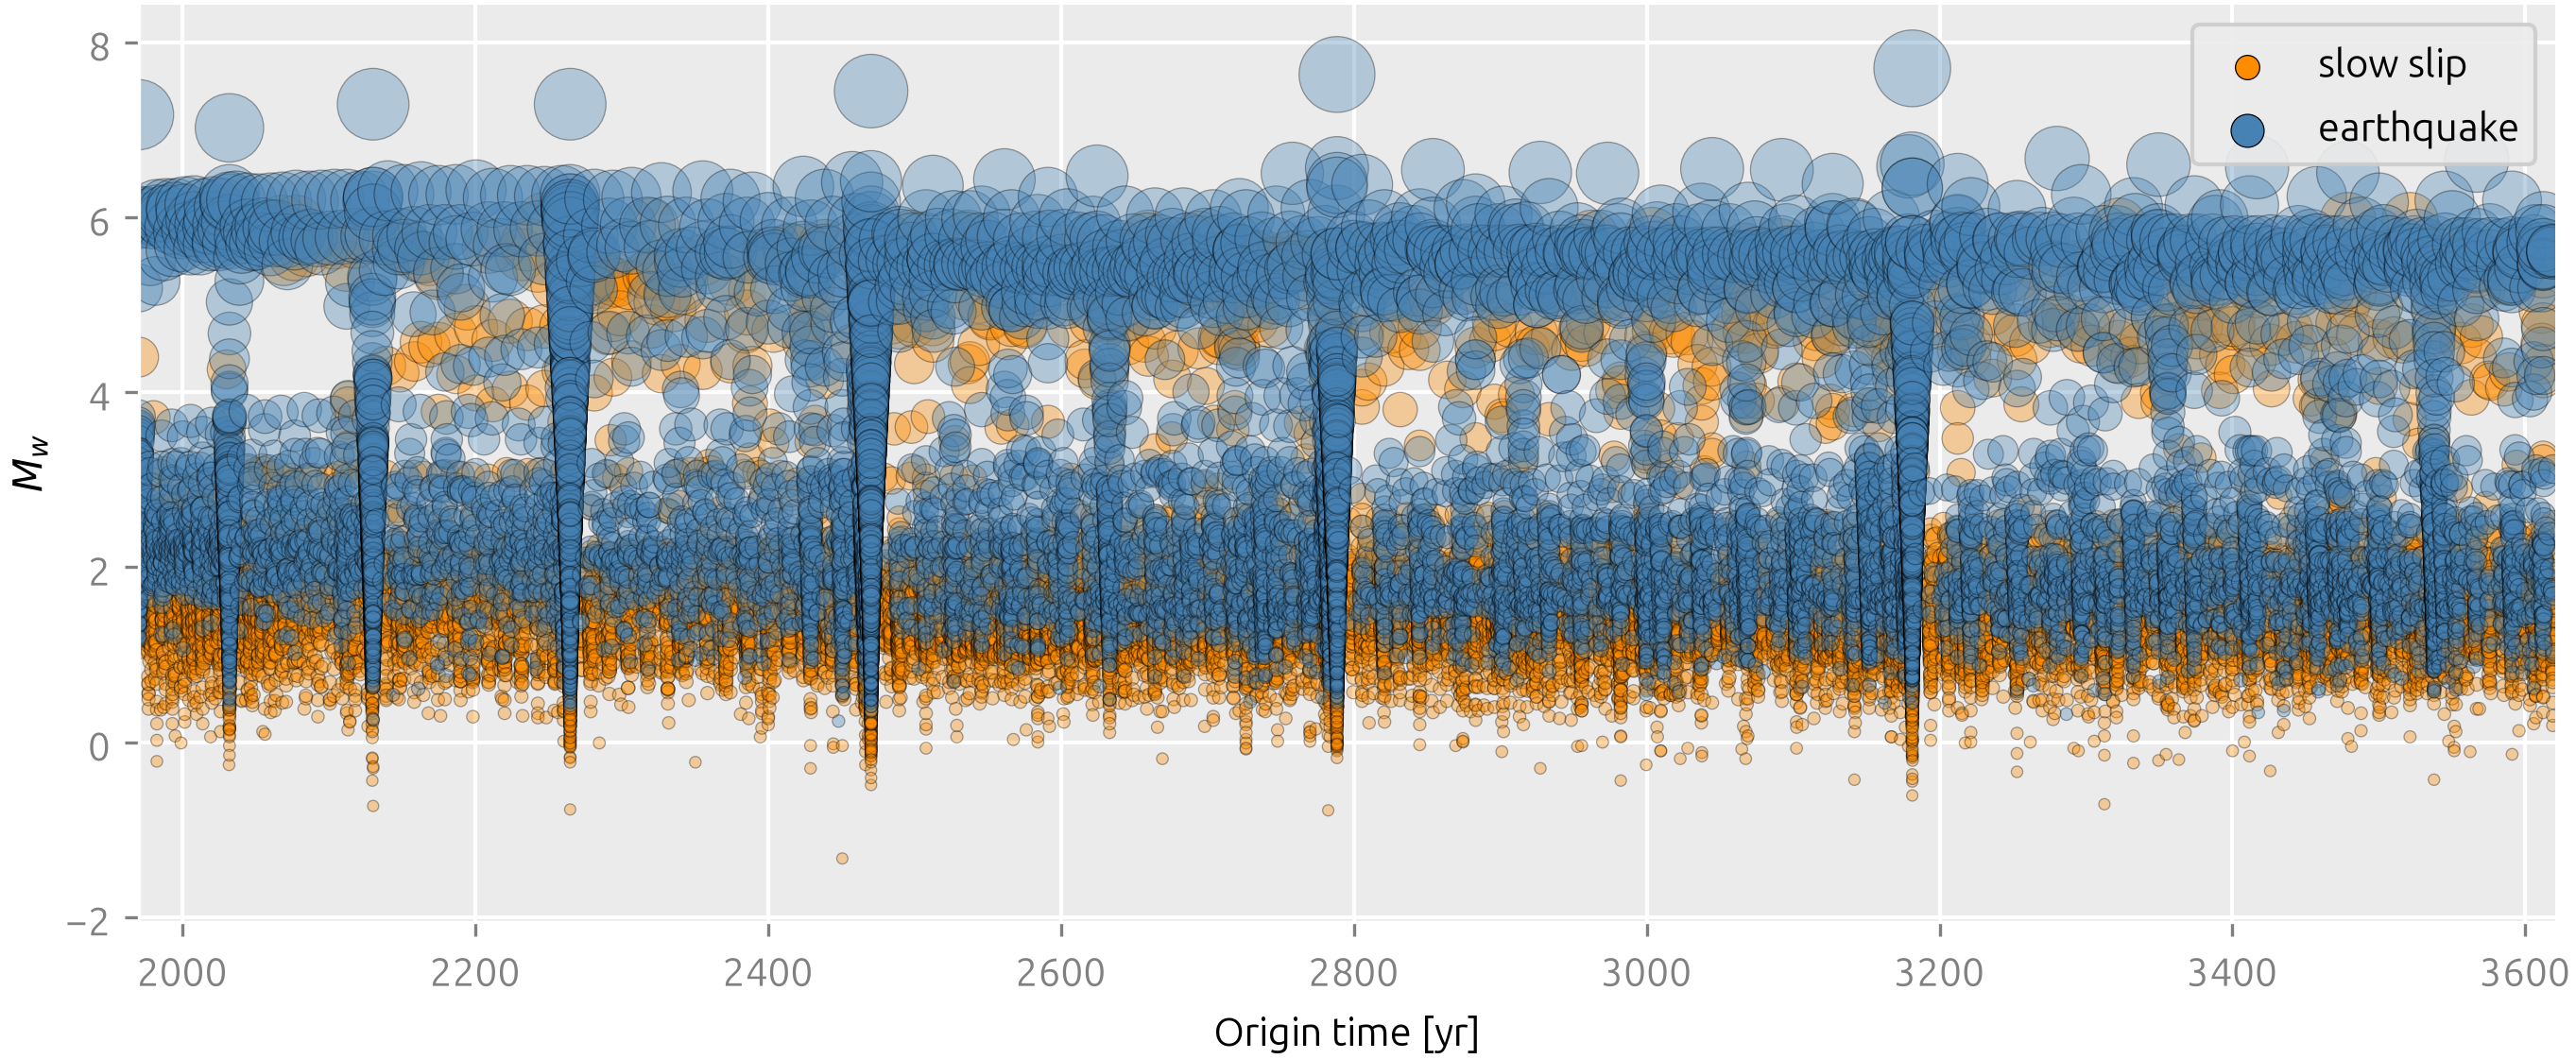
\includegraphics[width=0.95\textwidth]{./figures/plot_temporal}
		\caption*{\scriptsize Magnitude versus time. Large events recur quasi-periodically
		and are followed by triggered cascades.}
		\end{figure}
	}
	\only<2>{
		\begin{columns}[t]
			\column{.5\textwidth}
			\begin{figure}
			\vspace*{-0.3cm}
			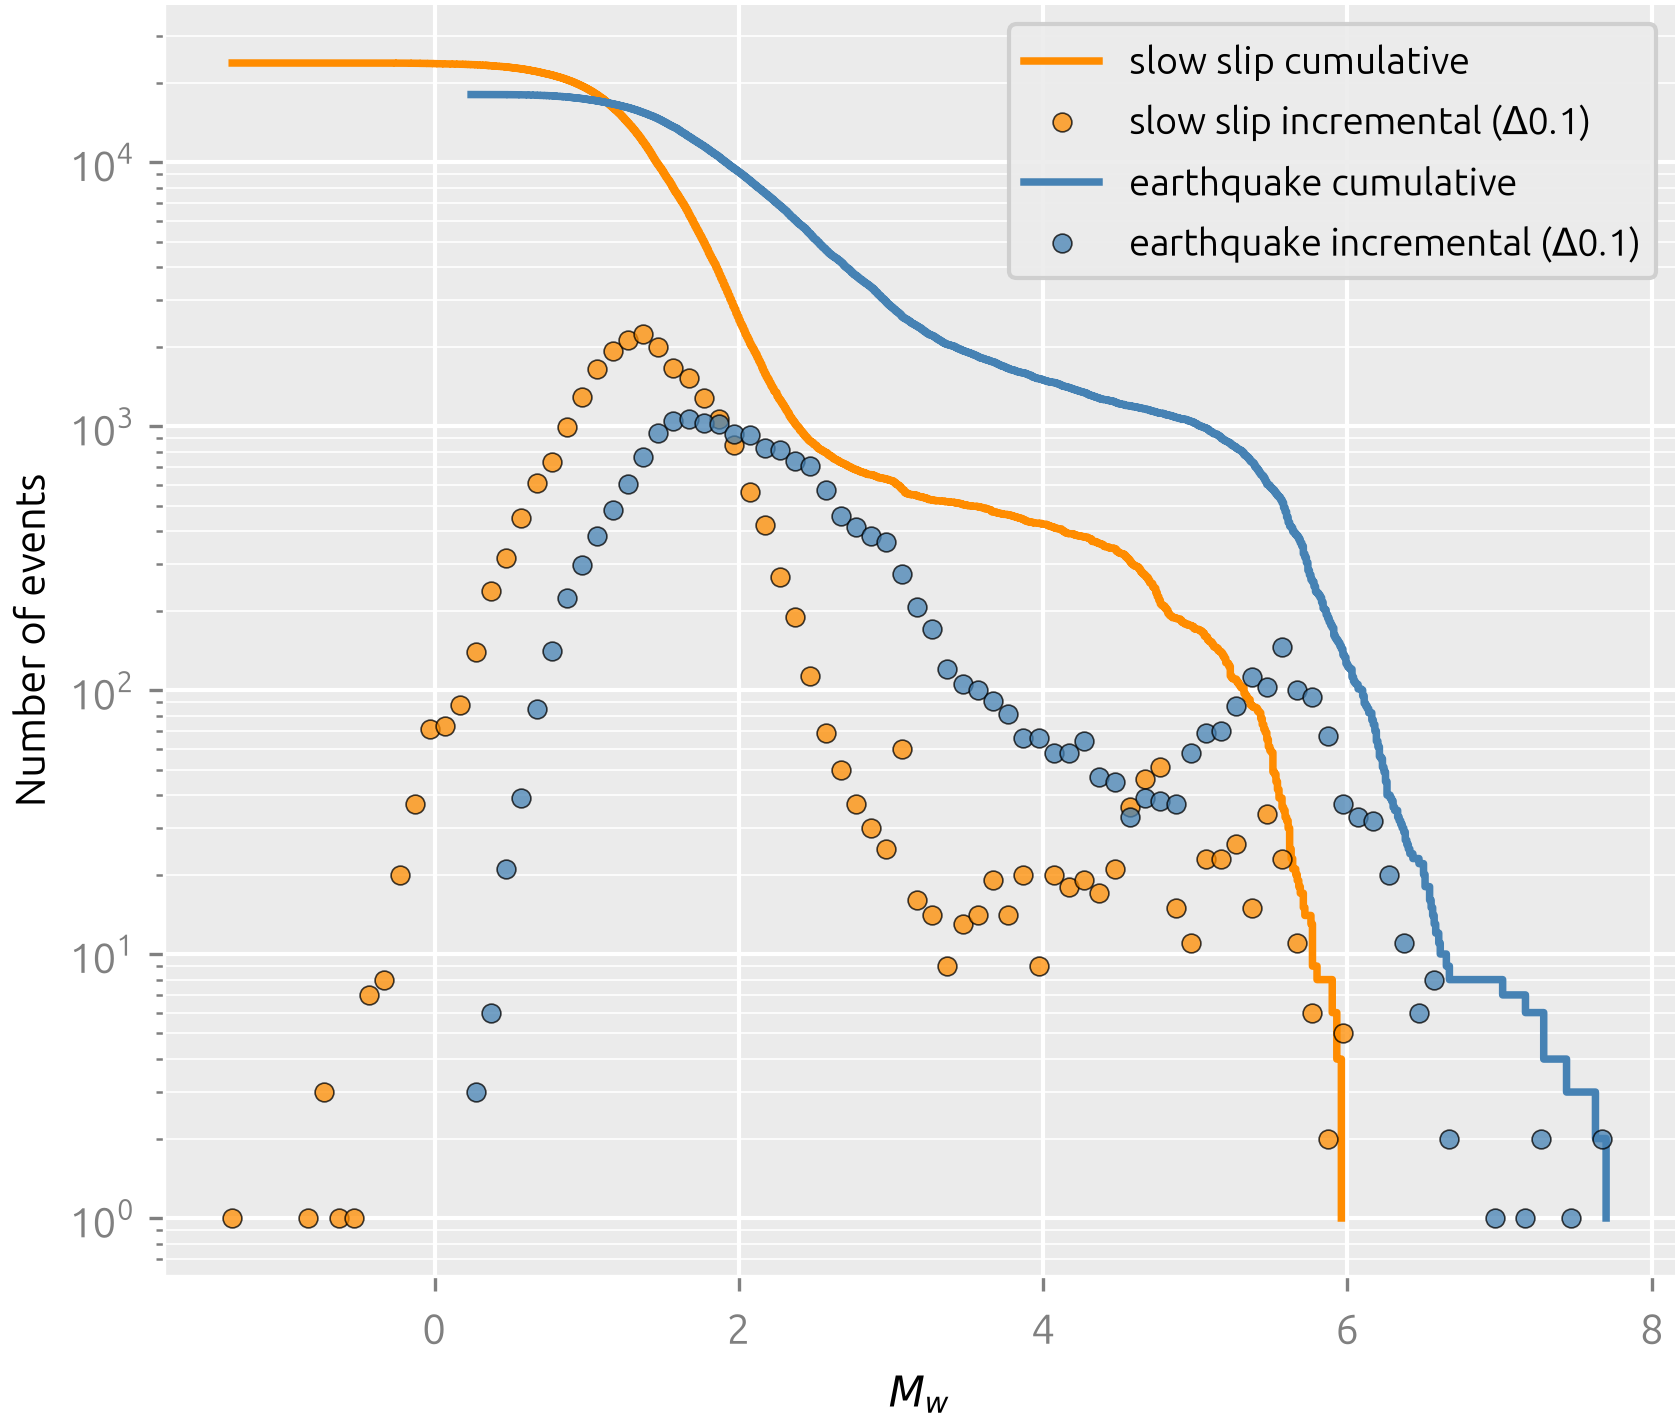
\includegraphics[width=1\textwidth]{./figures/plot_fmd}
			\caption*{\scriptsize Frequency--magnitude distribution: incremental (dots) and
			cumulative (lines).}
			\end{figure}
			\column{.5\textwidth}
			\begin{figure}
			\vspace*{-0.3cm}
			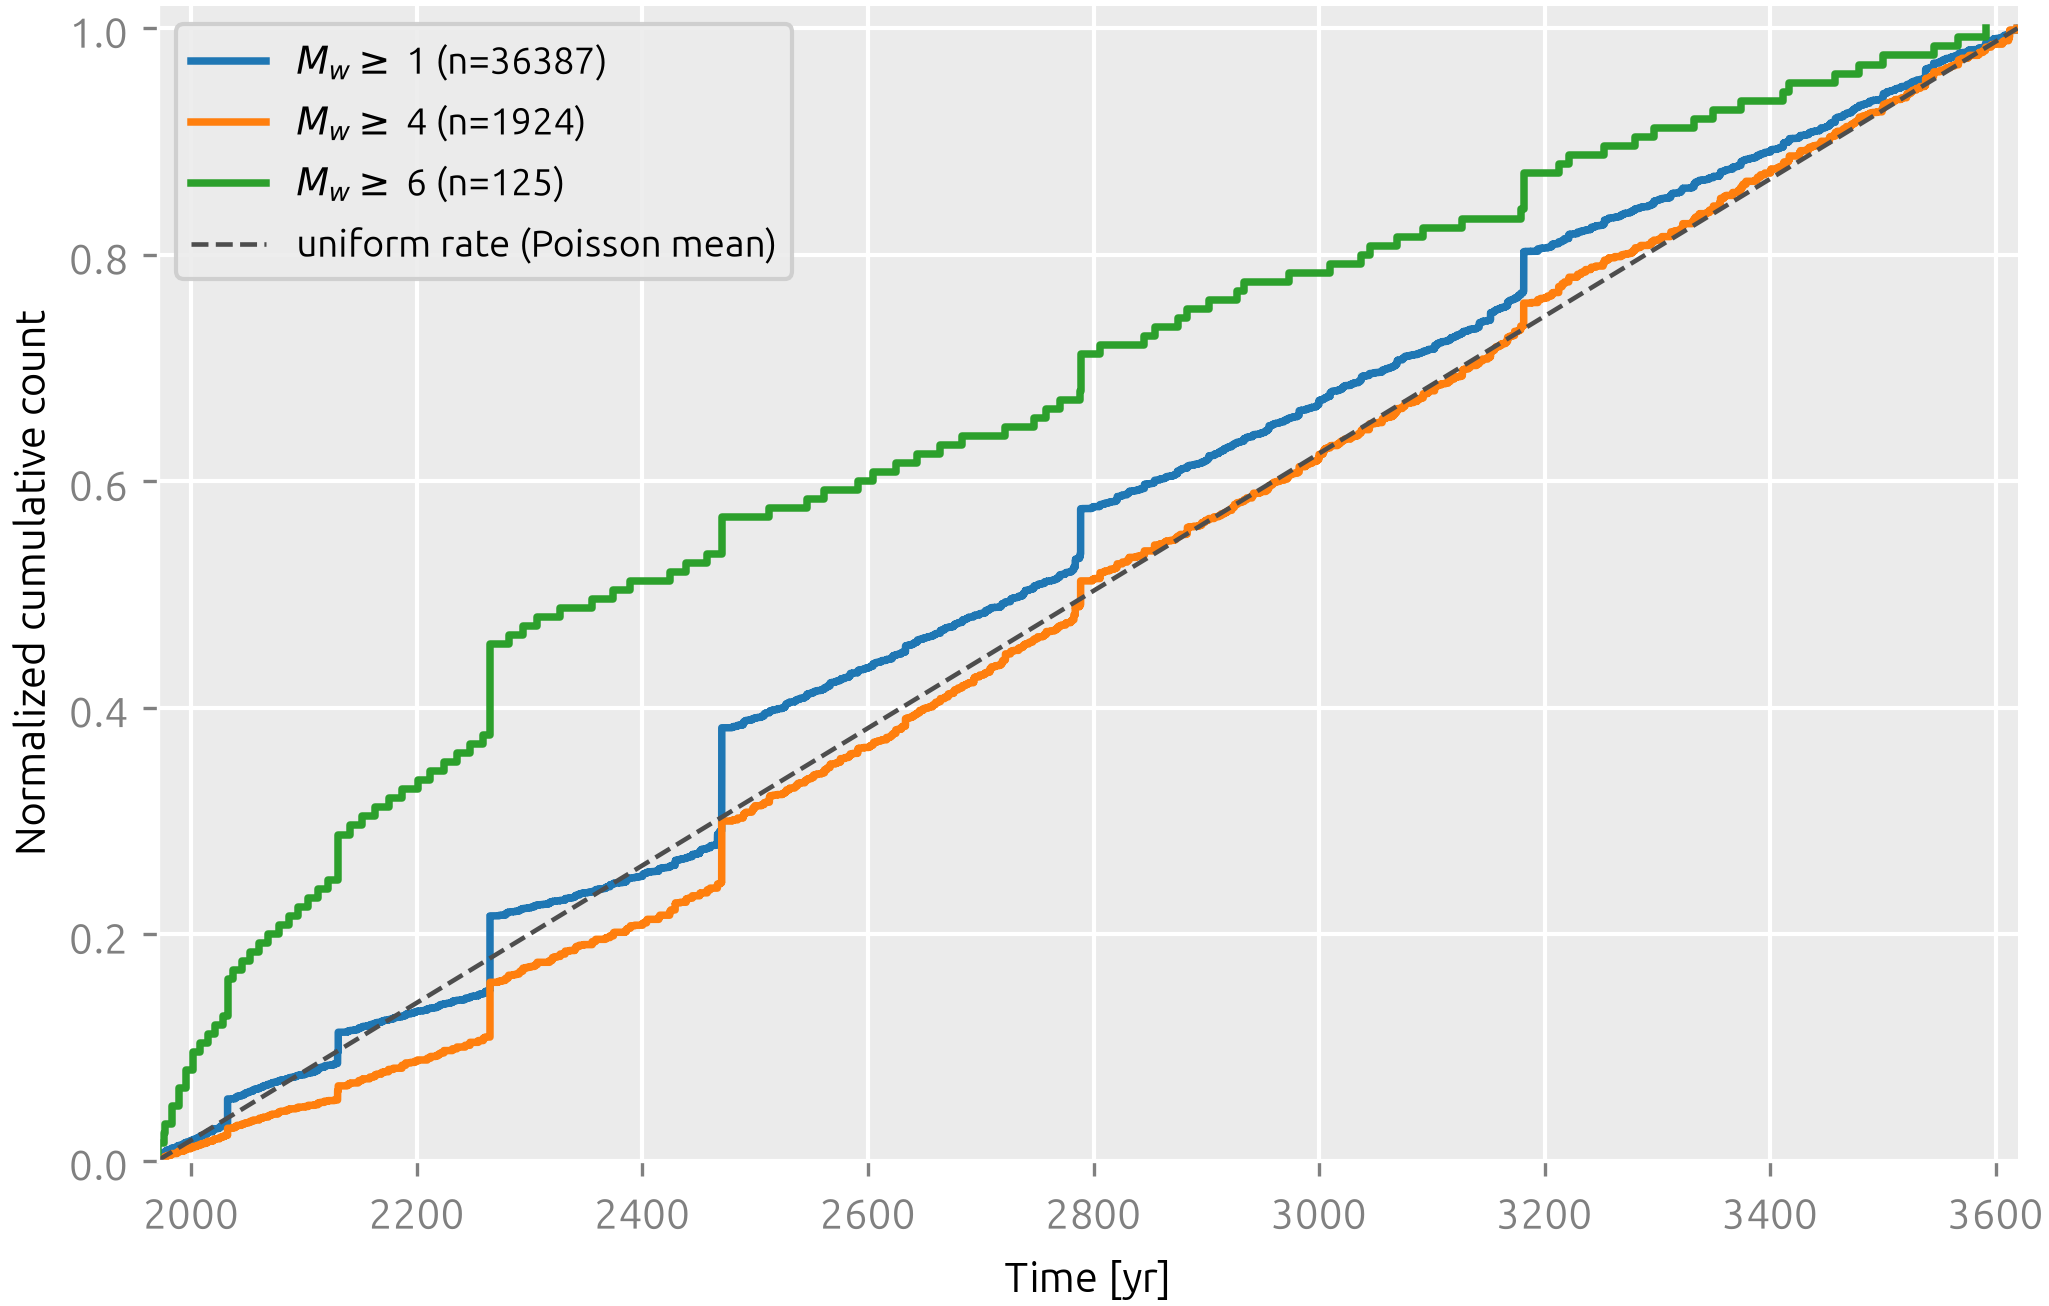
\includegraphics[width=1\textwidth]{./figures/plot_cumulative}
			\caption*{\scriptsize Normalized cumulative count against the uniform-rate
			(Poisson) expectation.}
			\end{figure}
		\end{columns}
	}
\end{frame}
\begin{frame}[t]
	\frametitle{Spatial distribution}
			\begin{figure}
			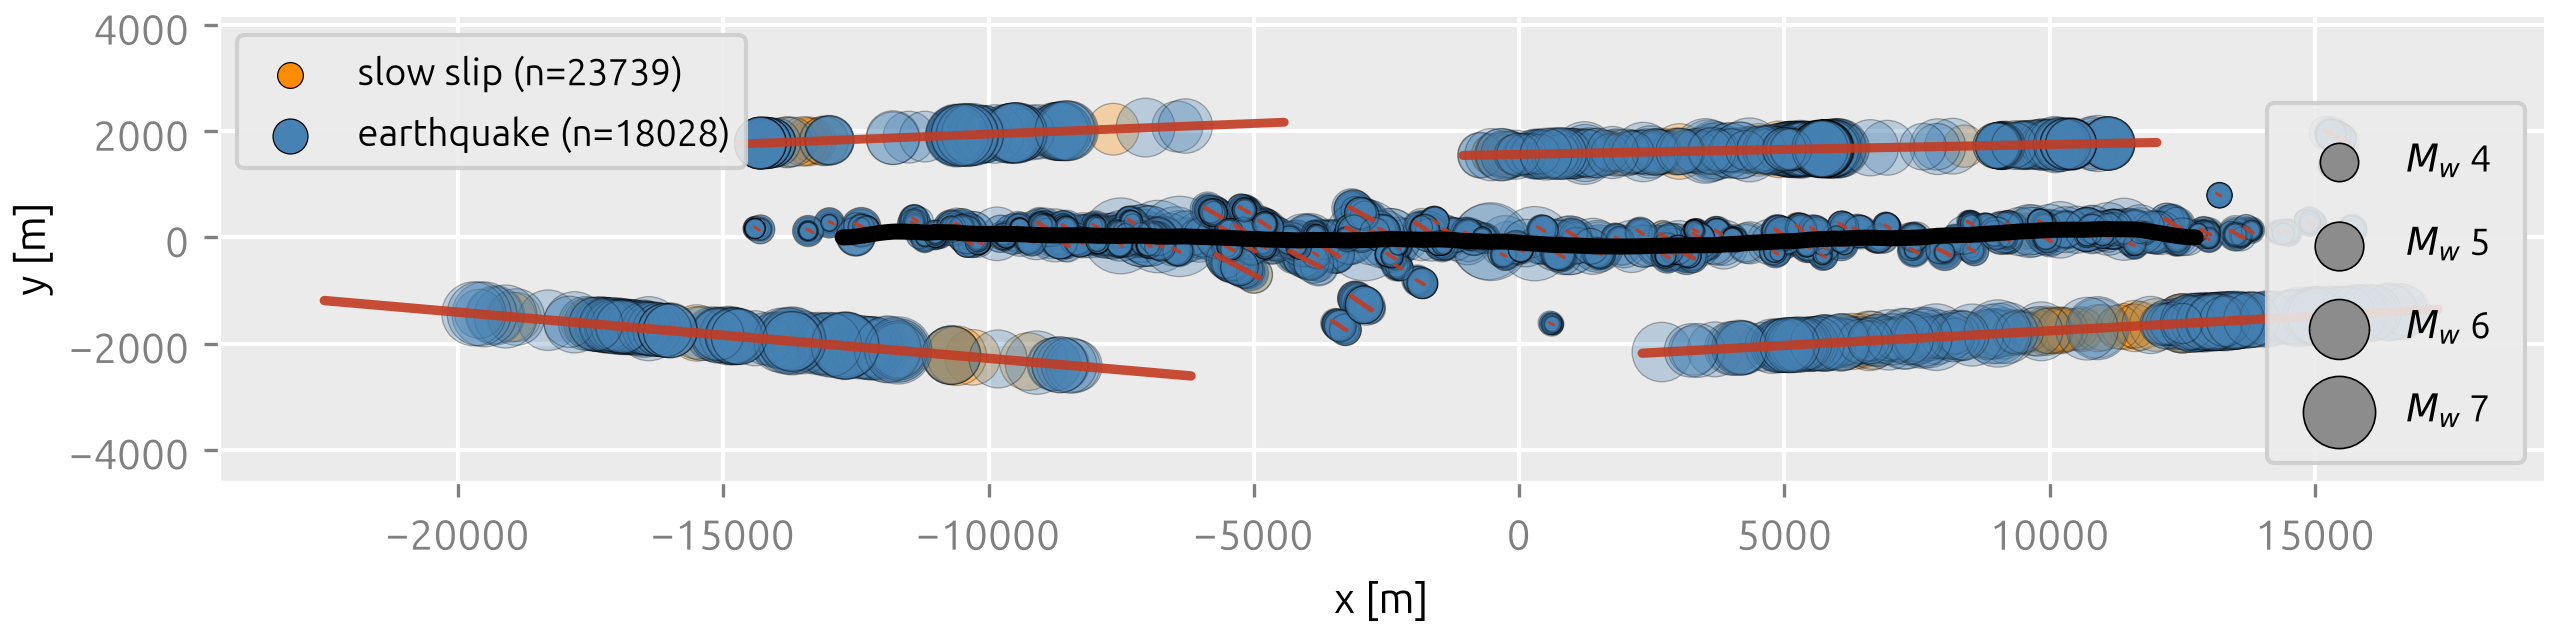
\includegraphics[width=0.95\textwidth]{./figures/plot_spatial}
			\caption*{\scriptsize Epicenters of the synthetic catalog over the fault network.
			Marker size scales with magnitude.}
			\end{figure}
\end{frame}
%% ------------------------------------------------------------------
%% PART 4 - From catalog to hazard
%% ------------------------------------------------------------------

\begin{frame}[t]
	\frametitle{From the catalog to hazard}

	\begin{columns}[t]
		\column{.55\textwidth}
	\begin{enumerate}\small
		\item<1-> Kep events with
		      $M_w \geq 4$.
		\item<2-> Sample $B$ overlapping windows of
		      $\Delta = 50$ years. \textbf{Each window is one possible
		      scenario.}
		\item<3-> Propagate shaking for every event with a Ground-Motion Model (Boore \& Atkinson,
		      2008), sampling its variability.
		\item<4-> Take the maximum PGA of each window.
		\item<5-> The hazard curve is the empirical survival function
		      of those maxima.
	\end{enumerate}

	\vspace{0.2cm}
	\only<5>{
	\begin{exampleblock}{}
	\begin{equation*}
 \widehat{P}\bigl(\mathrm{IM} > y \text{ in } T\bigr)  = \frac{1}{N} \sum_{k=1}^{N} H\!\bigl(Y_{\max}^{(k)} - y\bigr)
	\end{equation*}
        where $N$ is the number of synthetic catalogs, $y$ is a given value of ground motion intensity (e.g., PGA) and $Y_{\max}^{(k)}$ is the maximum sampled ground motion of each synthetic catalog.
	\end{exampleblock}
	}
		\column{.45\textwidth}

	\end{columns}
\end{frame}

\begin{frame}[t]
	\frametitle{Hazard from a physics-based catalog}

	\only<1>{
		\begin{figure}
		\vspace*{-0.3cm}
		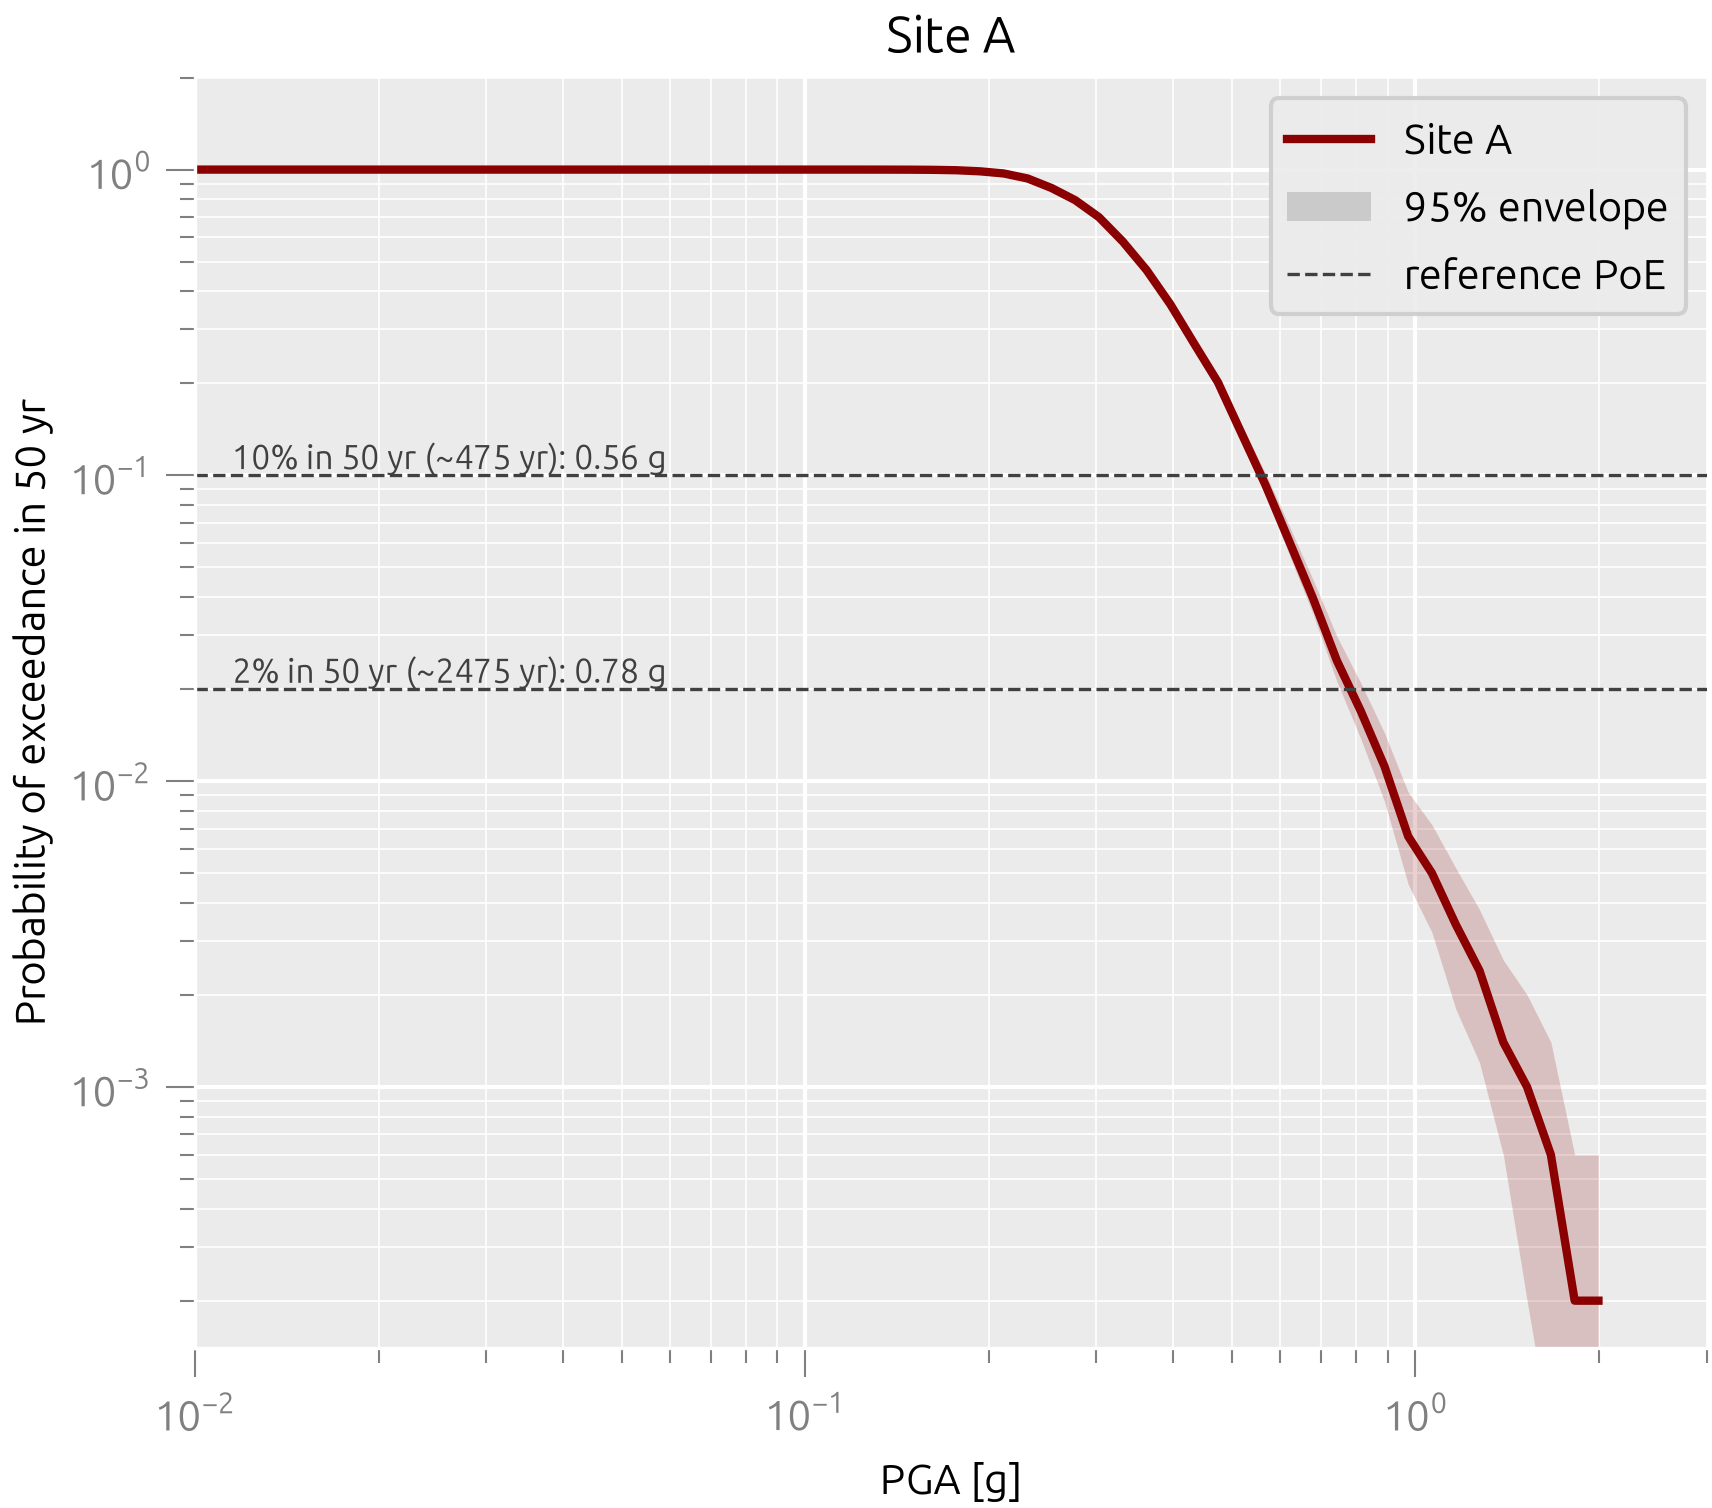
\includegraphics[width=0.55\textwidth]{./figures/hazard_curves}
		\caption*{\scriptsize Hazard curve at a near-fault site. Shaded: 95\% bootstrap
		envelope. Dashed: reference exceedance probabilities. The curve
		flattens at the resolution floor $1/B$ set by the number of
		windows.}
		\end{figure}
	}
	\only<2>{
		\begin{figure}
		\vspace*{-0.3cm}
		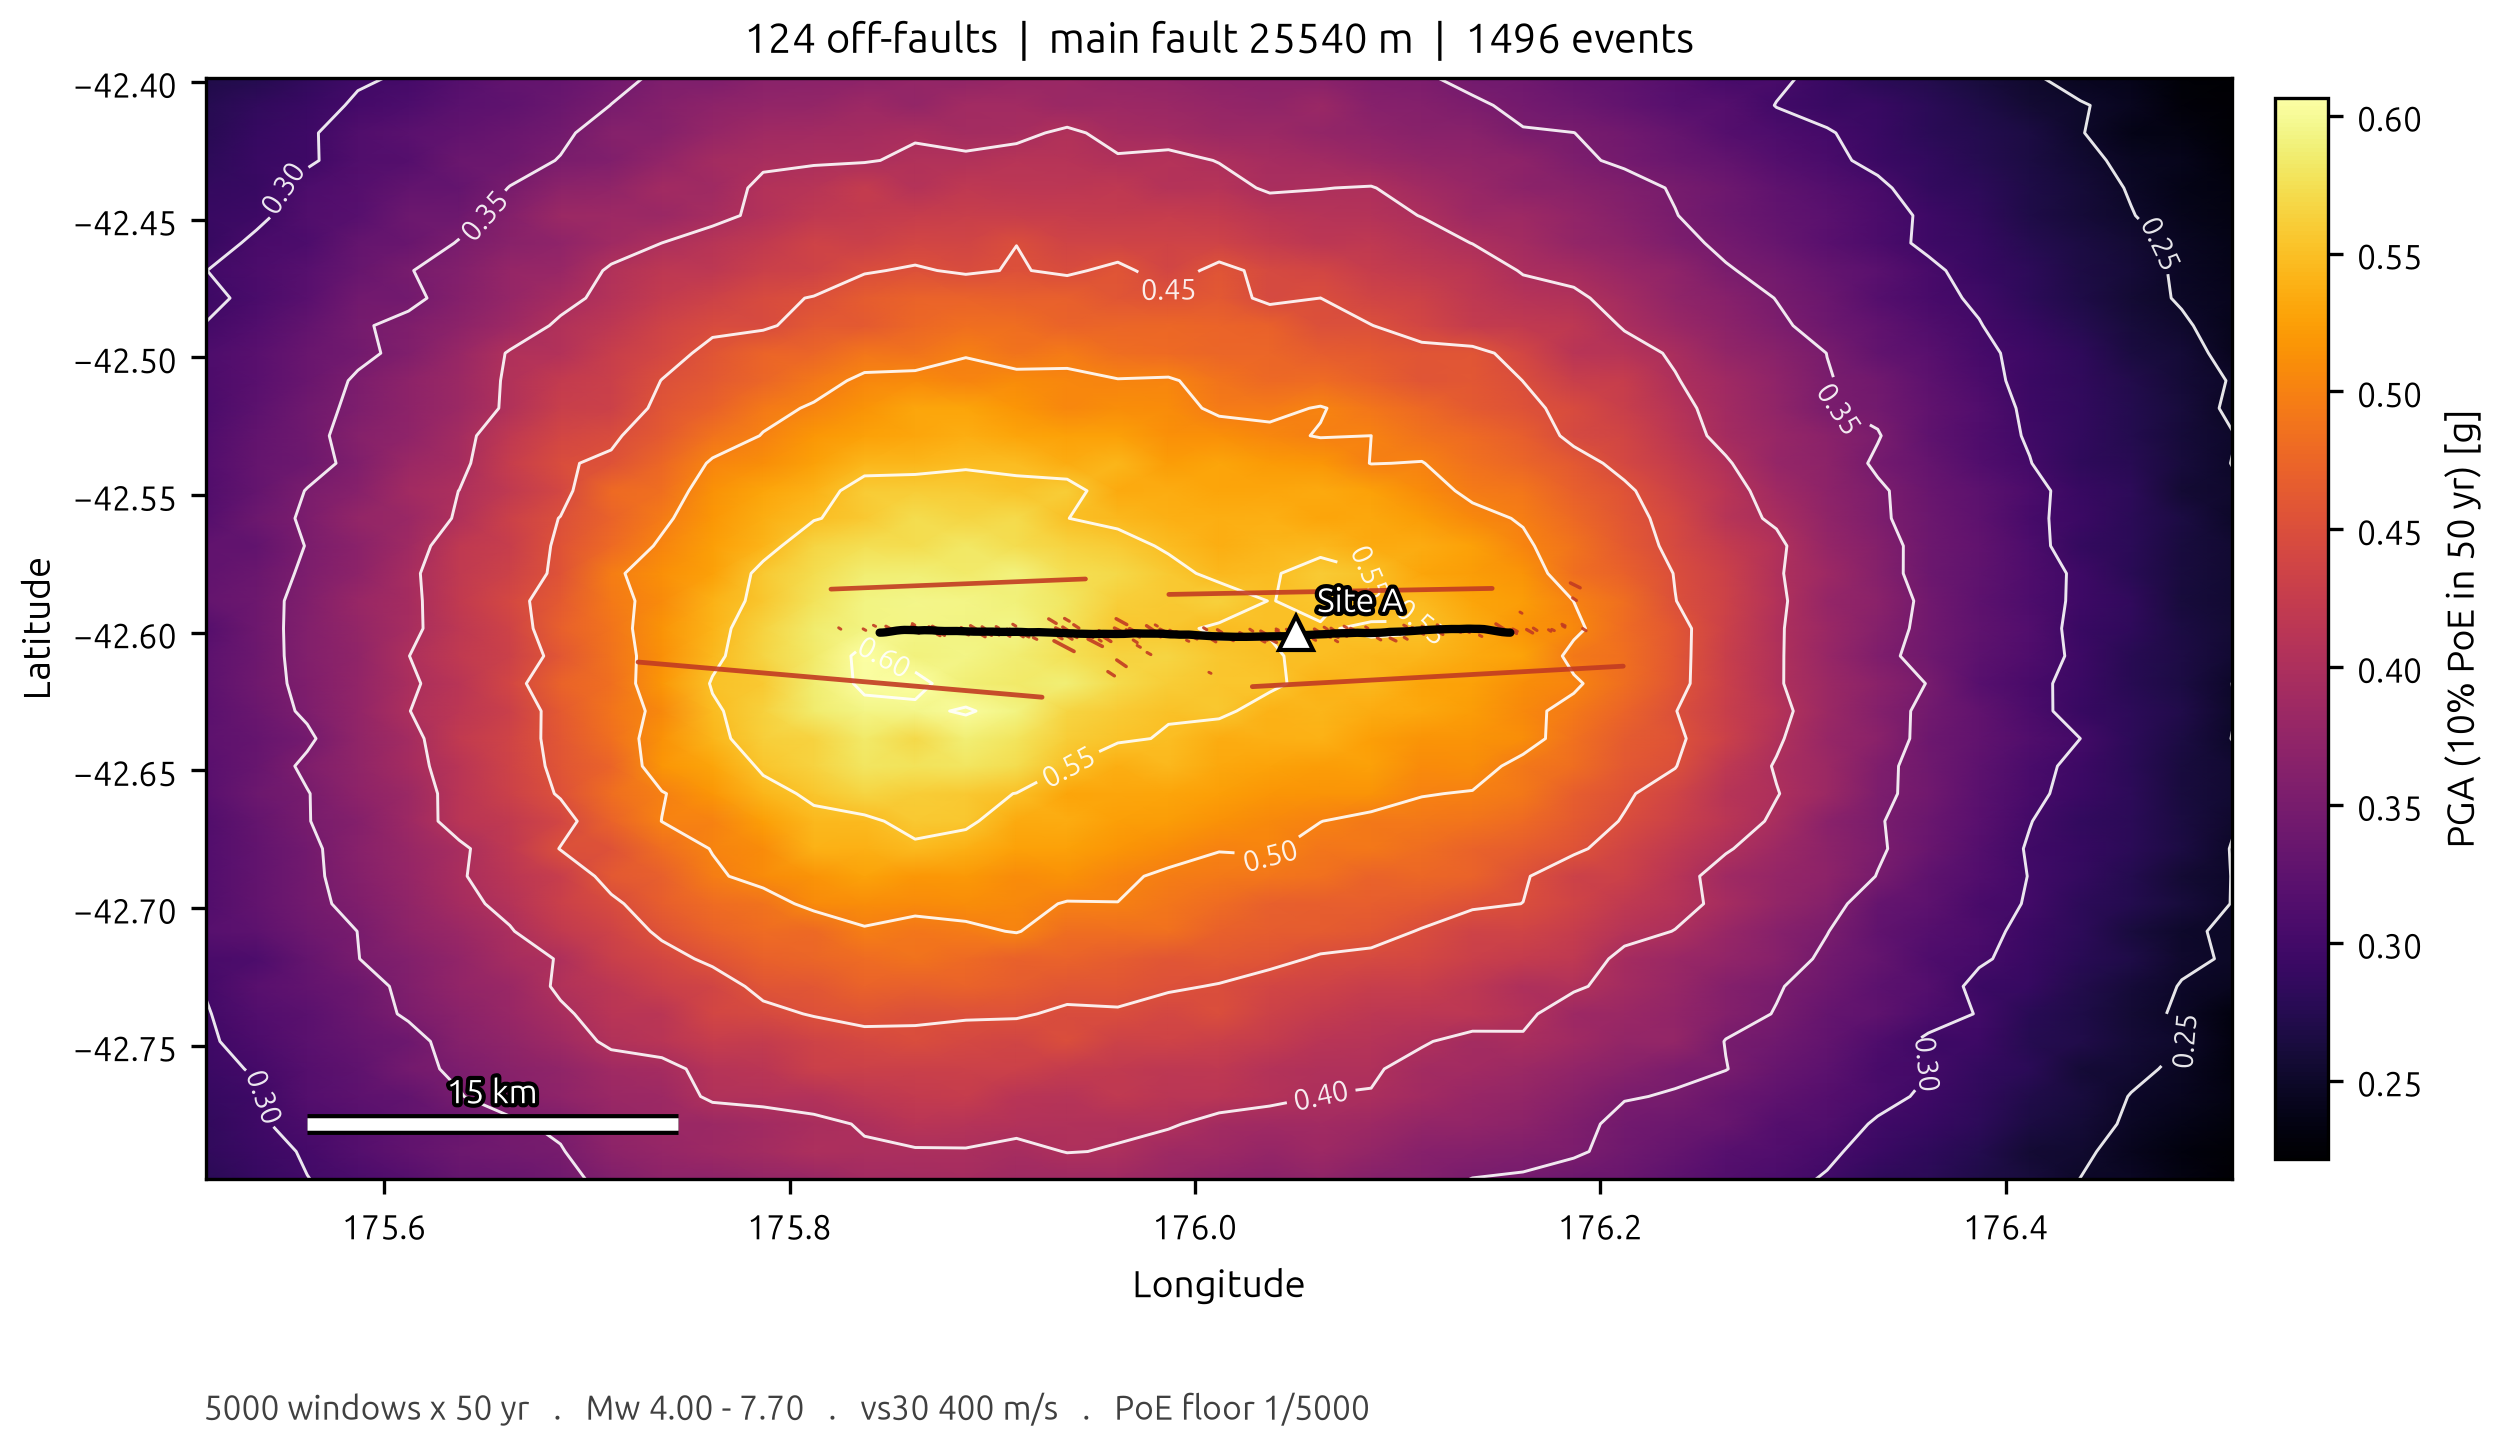
\includegraphics[width=0.95\textwidth]{./figures/hazard_map}
		\caption*{\scriptsize Hazard map from the synthetic catalog: PGA with 10\%
		probability of exceedance in 50 years. Main fault in black,
		subsidiary faults in red.}
		\end{figure}
	}
\end{frame}



%% ------------------------------------------------------------------
%% PART 3 - The synthetic catalog
%% ------------------------------------------------------------------

\begin{frame}[t]
	\frametitle{Synthetic catalogs with VEGA}

	\begin{columns}[t]
		\column{.2\textwidth}

		\column{.6\textwidth}
		\begin{figure}
		\vspace*{-0.7cm}
		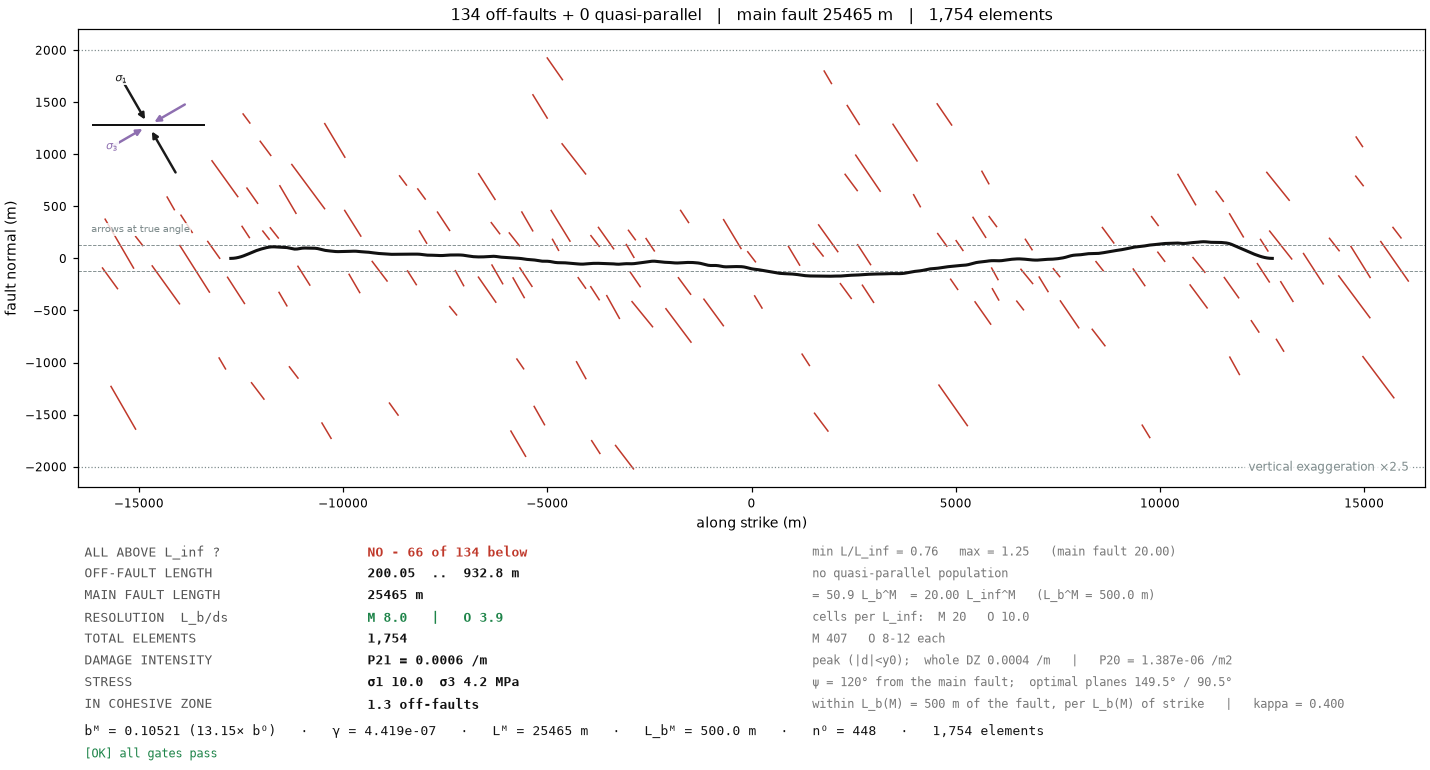
\includegraphics[width=1\textwidth]{./figures/fault_v6b}
		\caption*{\scriptsize Fault network generated for the experiment.}
		\end{figure}
	\end{columns}
\end{frame}

\begin{frame}[t]
	\frametitle{The resulting catalog}

	\only<1>{
		\begin{figure}
		\vspace*{-0.3cm}
		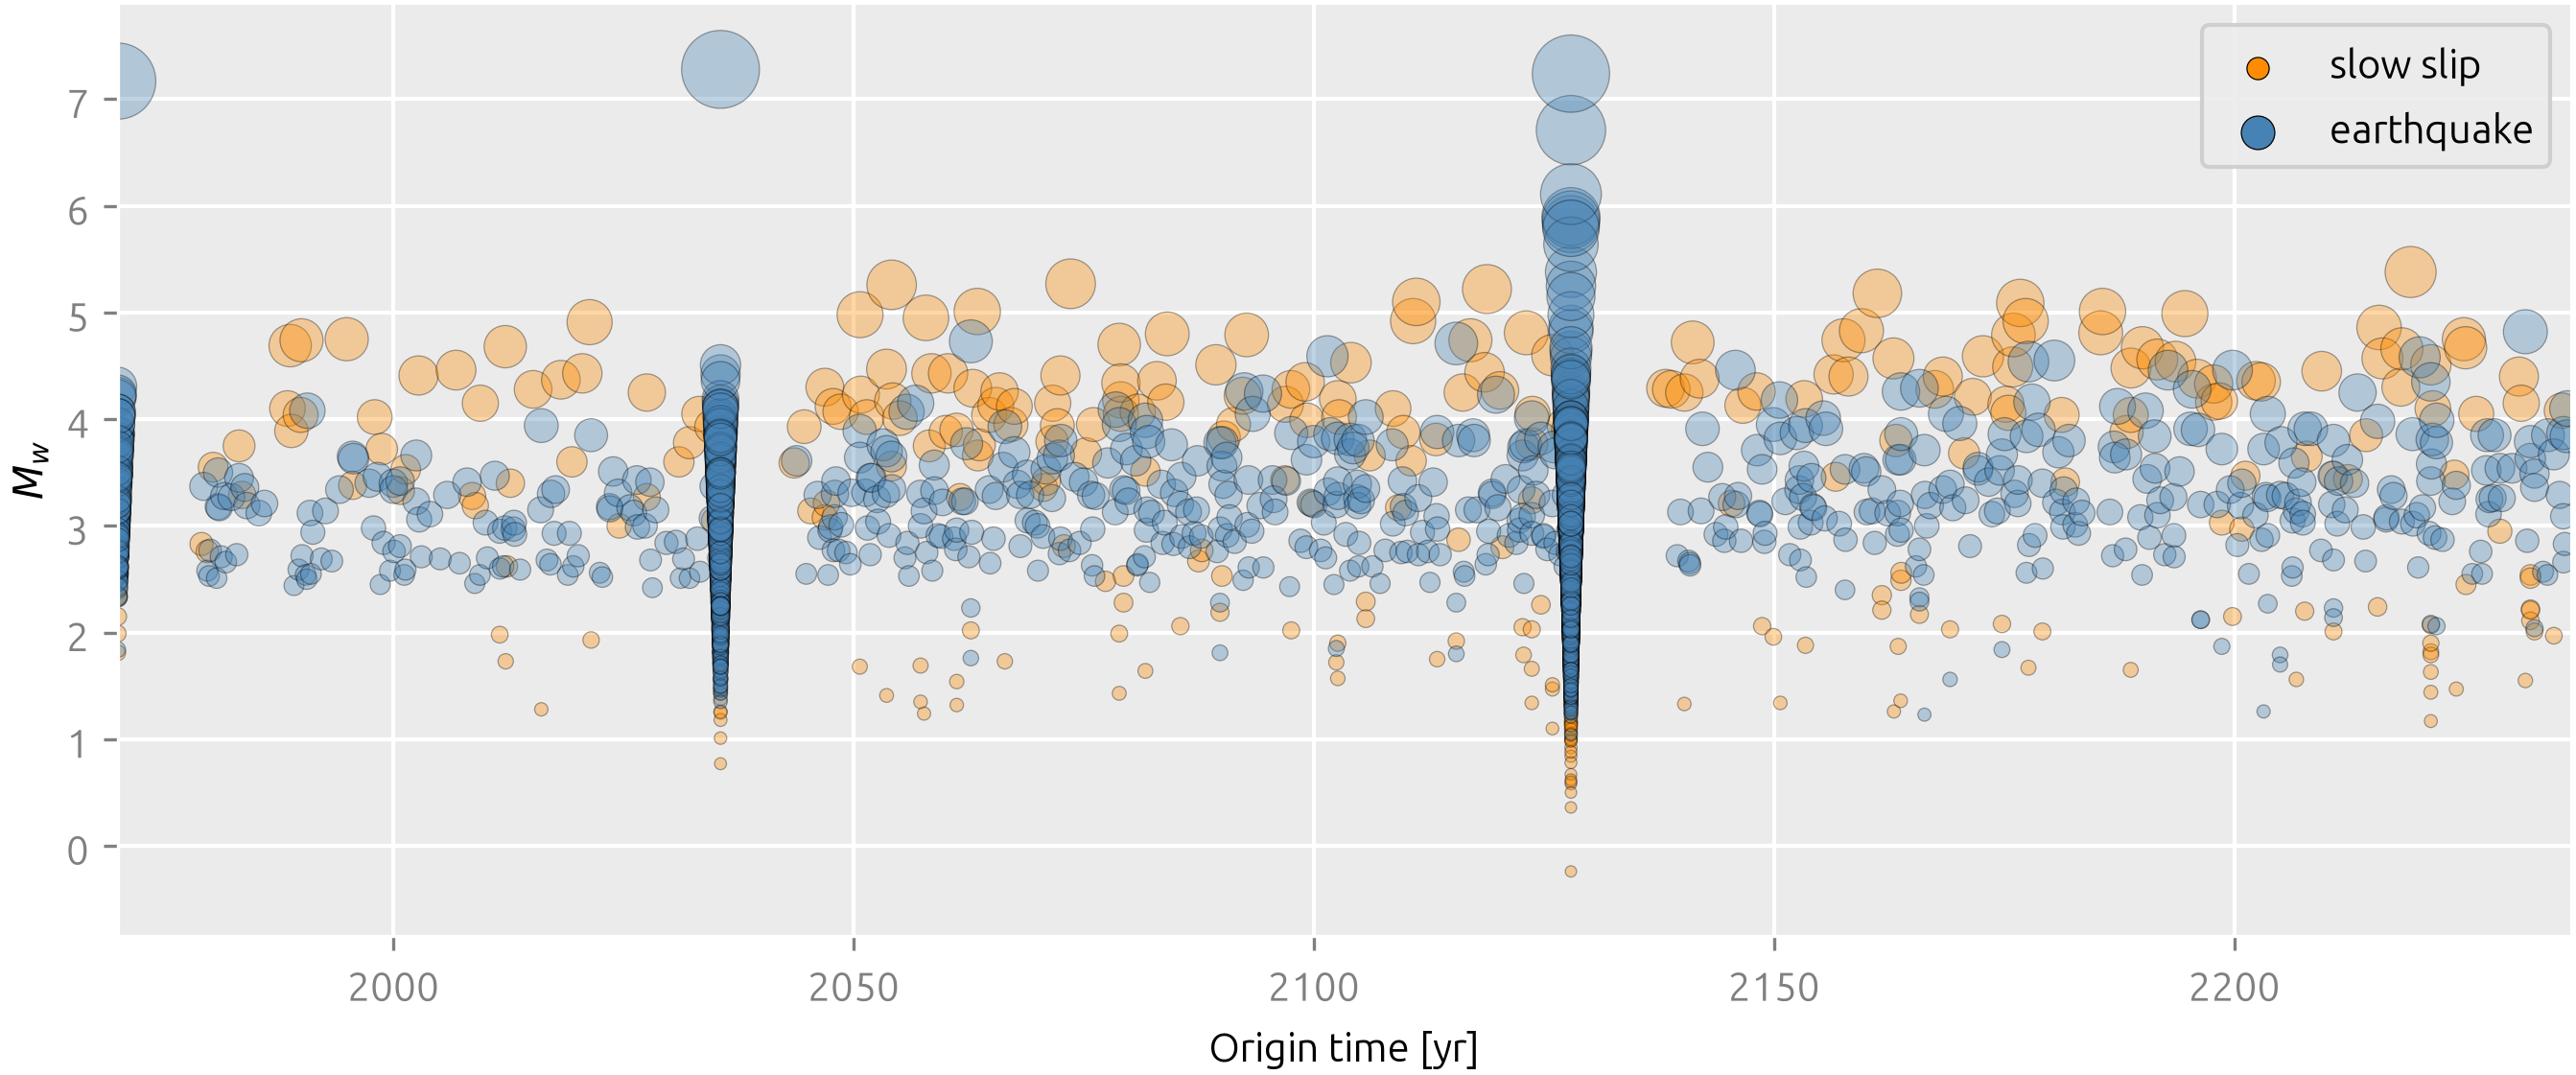
\includegraphics[width=0.95\textwidth]{./figures/plot_temporalb}
		\caption*{\scriptsize Magnitude versus time. Large events recur quasi-periodically
		and are followed by triggered cascades.}
		\end{figure}
	}
	\only<2>{
		\begin{columns}[t]
			\column{.5\textwidth}
			\begin{figure}
			\vspace*{-0.3cm}
			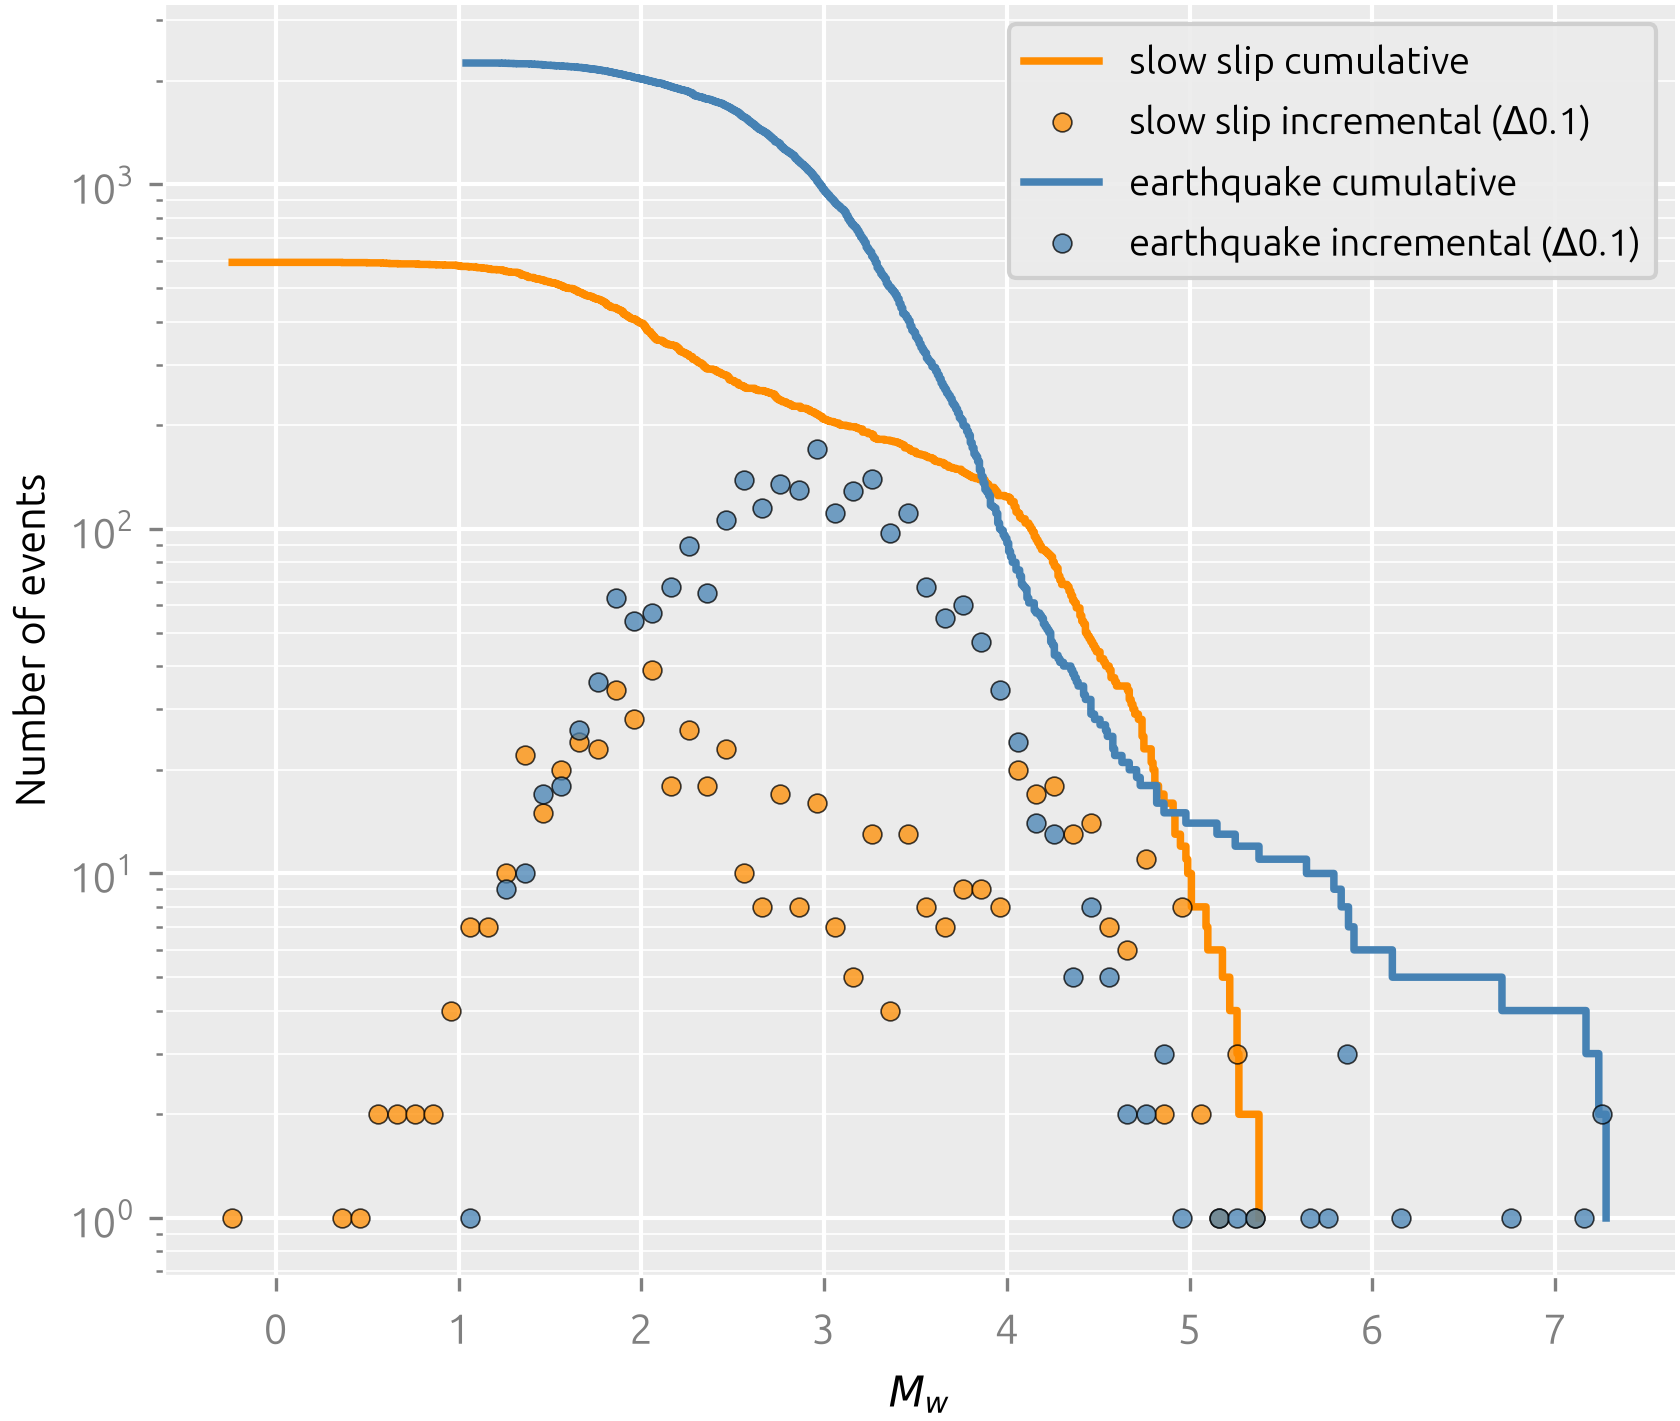
\includegraphics[width=1\textwidth]{./figures/plot_fmdb}
			\caption*{\scriptsize Frequency--magnitude distribution: incremental (dots) and
			cumulative (lines).}
			\end{figure}
			\column{.5\textwidth}
			\begin{figure}
			\vspace*{-0.3cm}
			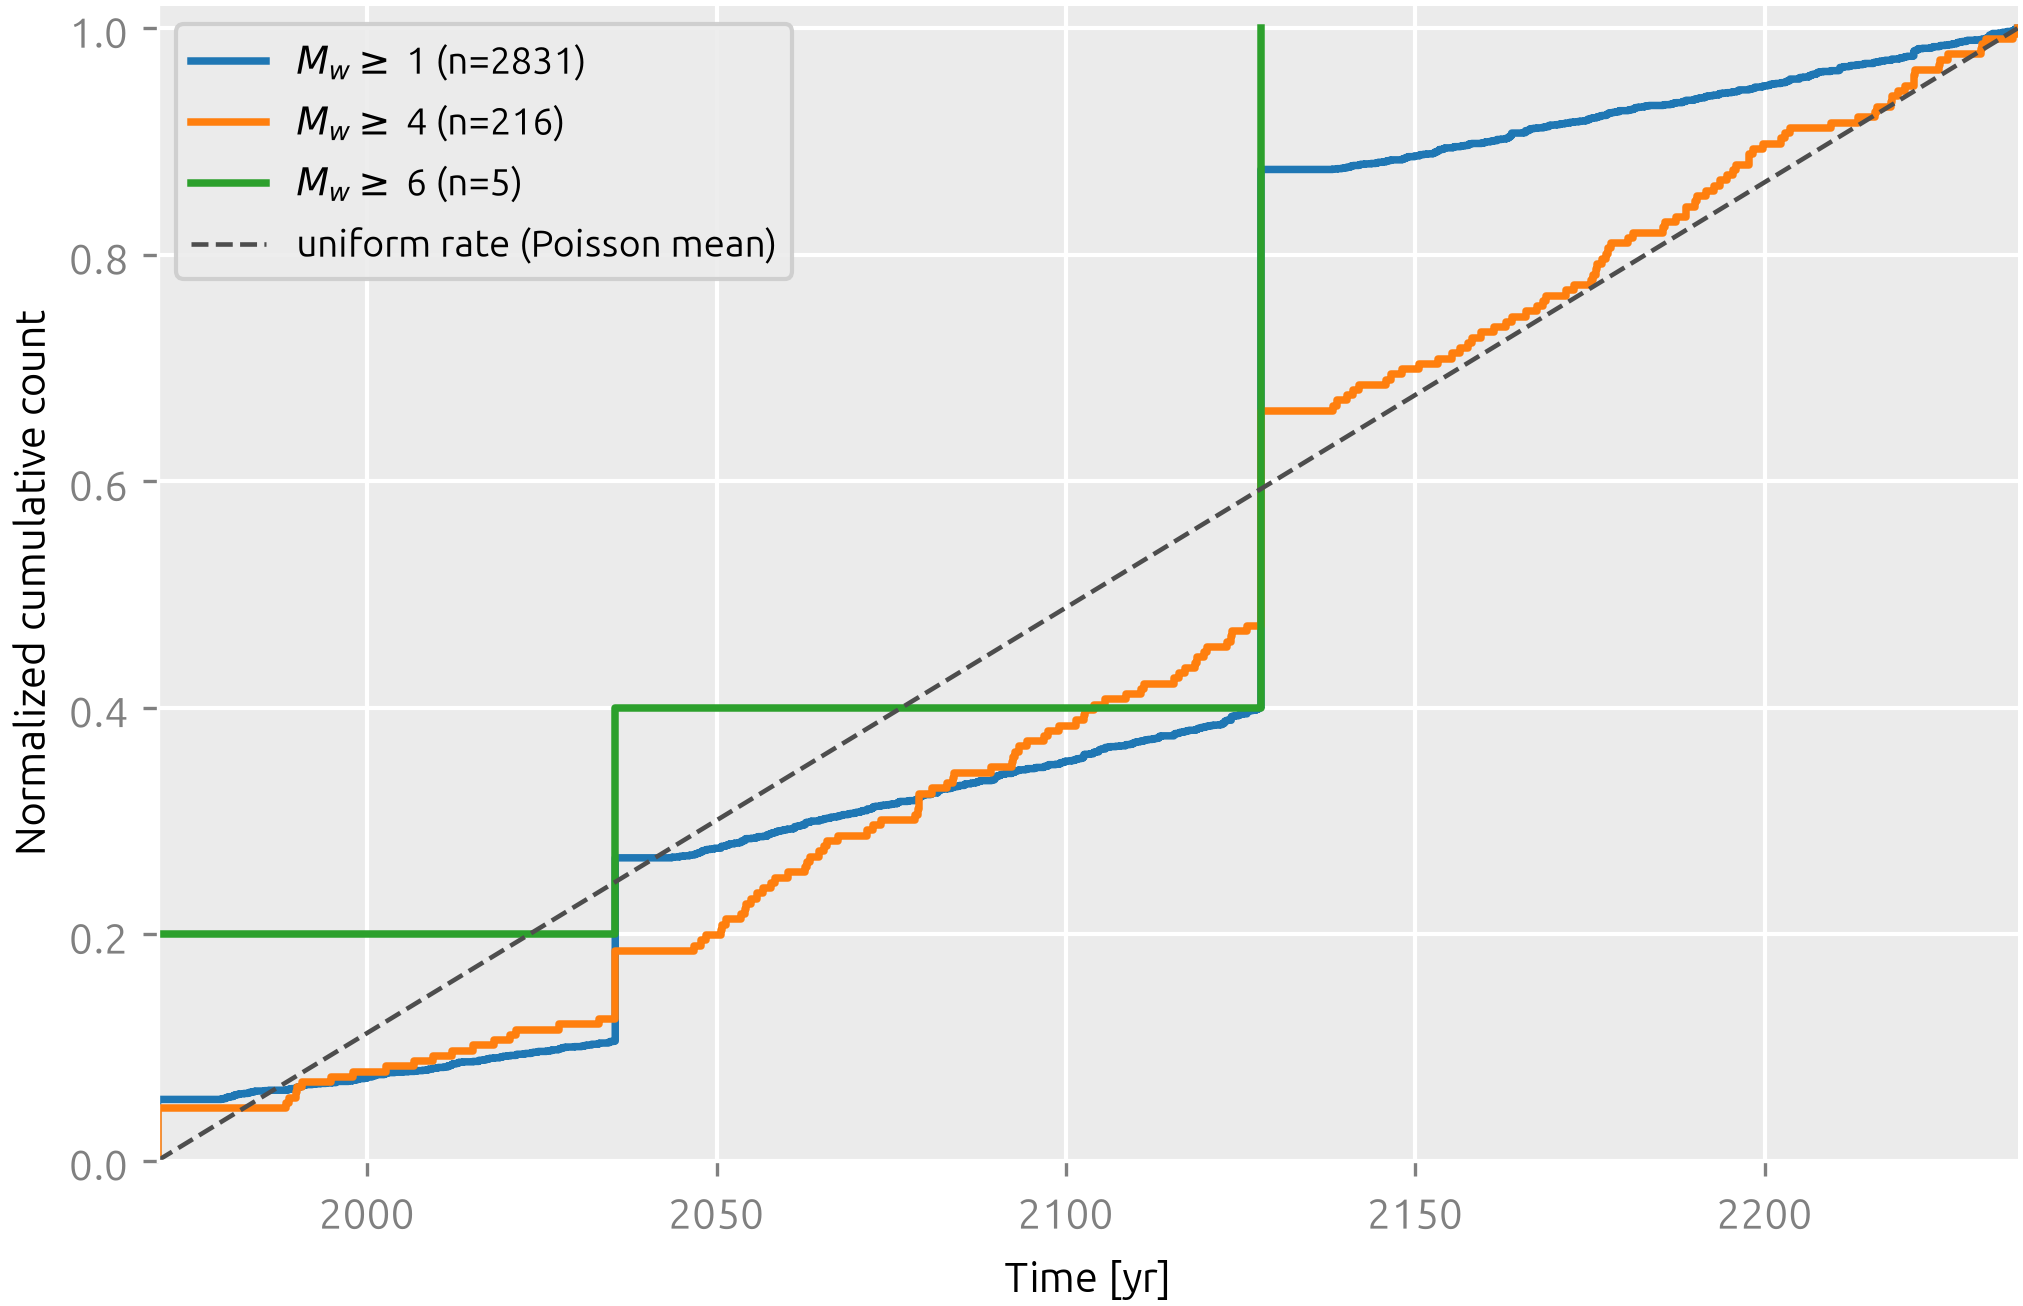
\includegraphics[width=1\textwidth]{./figures/plot_cumulativeb}
			\caption*{\scriptsize Normalized cumulative count against the uniform-rate
			(Poisson) expectation.}
			\end{figure}
		\end{columns}
	}
\end{frame}
\begin{frame}[t]
	\frametitle{Spatial distribution}
			\begin{figure}
			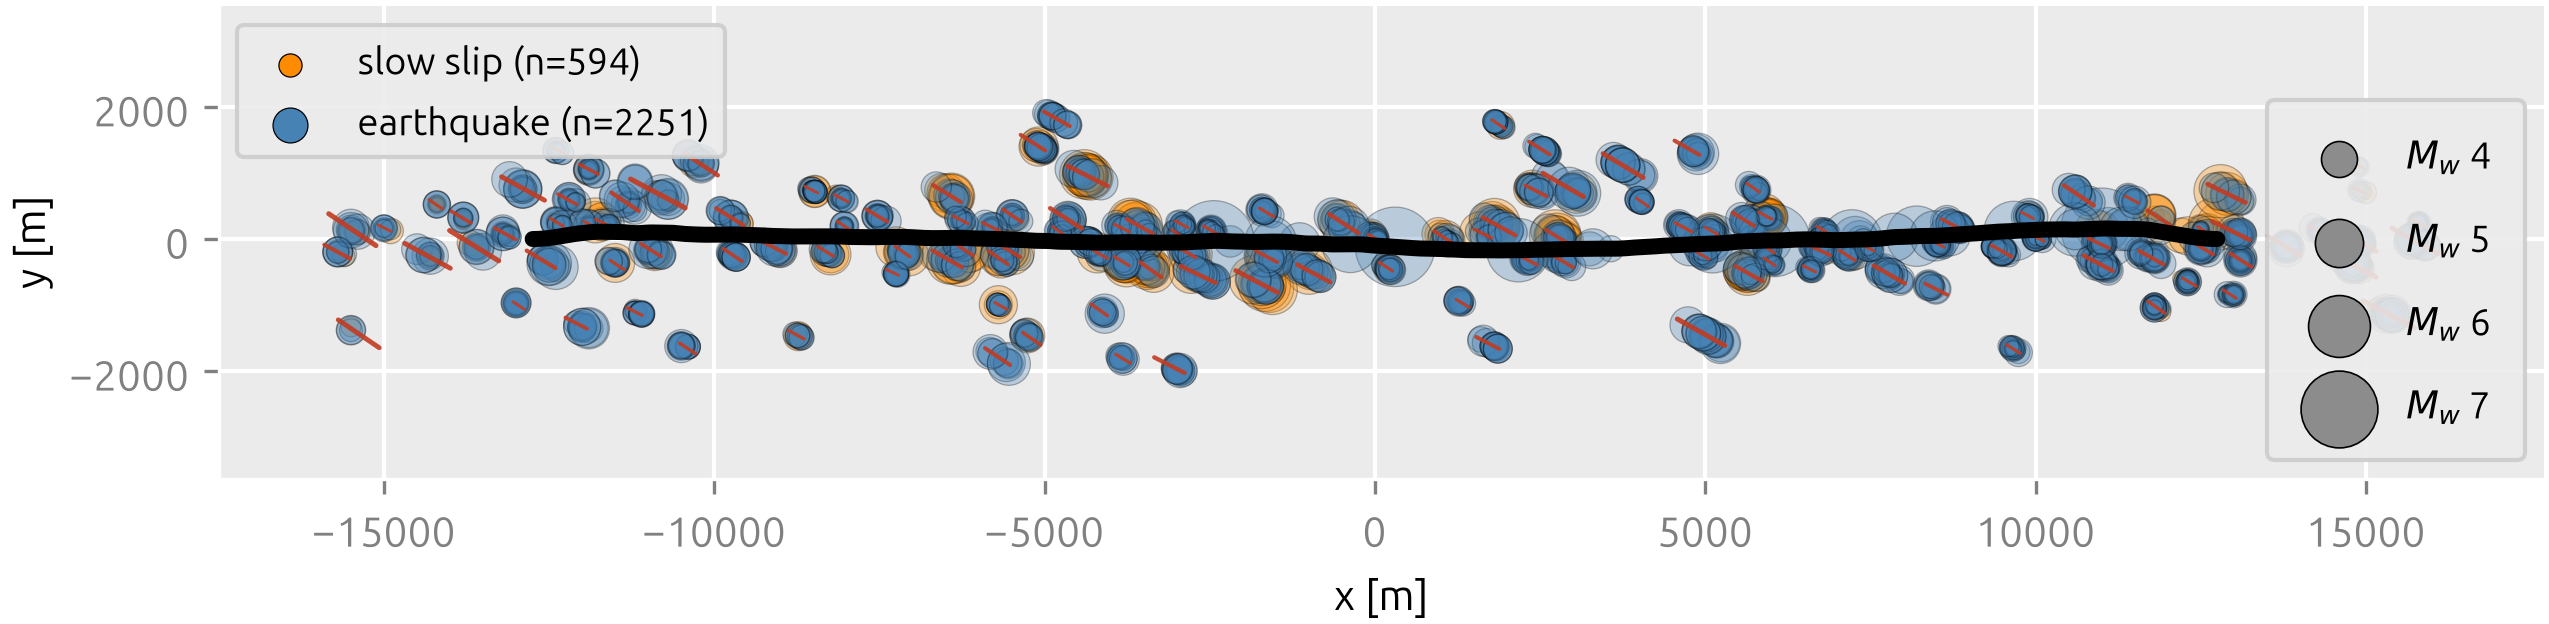
\includegraphics[width=0.95\textwidth]{./figures/plot_spatialb}
			\caption*{\scriptsize Epicenters of the synthetic catalog over the fault network.
			Marker size scales with magnitude.}
			\end{figure}
\end{frame}
%% ------------------------------------------------------------------
%% PART 4 - From catalog to hazard
%% ------------------------------------------------------------------

\begin{frame}[t]
	\frametitle{Hazard from a physics-based catalog}

	\only<1>{
		\begin{figure}
		\vspace*{-0.3cm}
		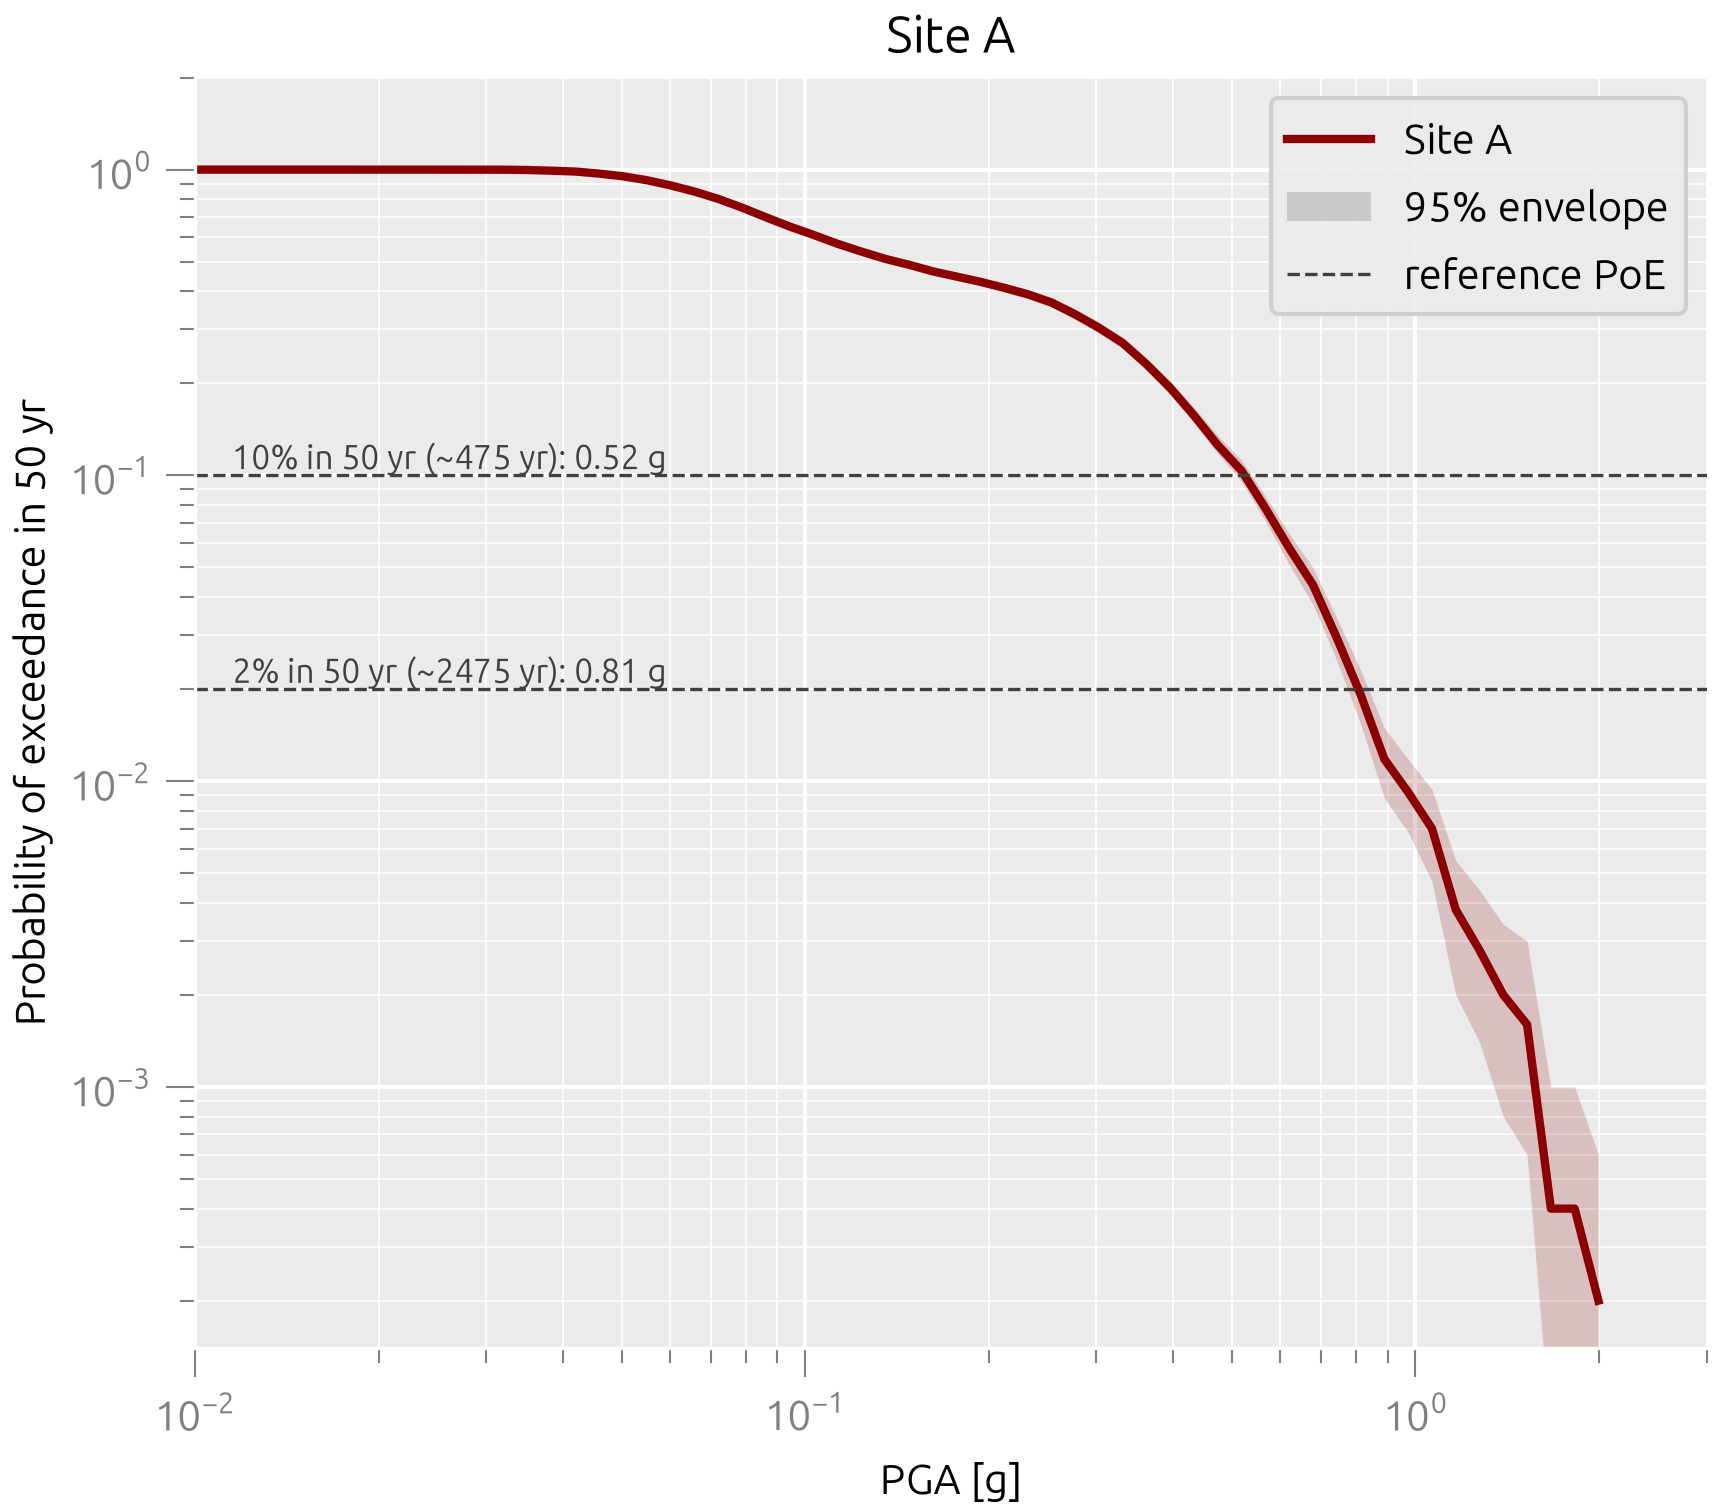
\includegraphics[width=0.55\textwidth]{./figures/hazard_curvesb}
		\caption*{\scriptsize Hazard curve at a near-fault site. Shaded: 95\% bootstrap
		envelope. Dashed: reference exceedance probabilities. The curve
		flattens at the resolution floor $1/B$ set by the number of
		windows.}
		\end{figure}
	}
	\only<2>{
		\begin{figure}
		\vspace*{-0.3cm}
		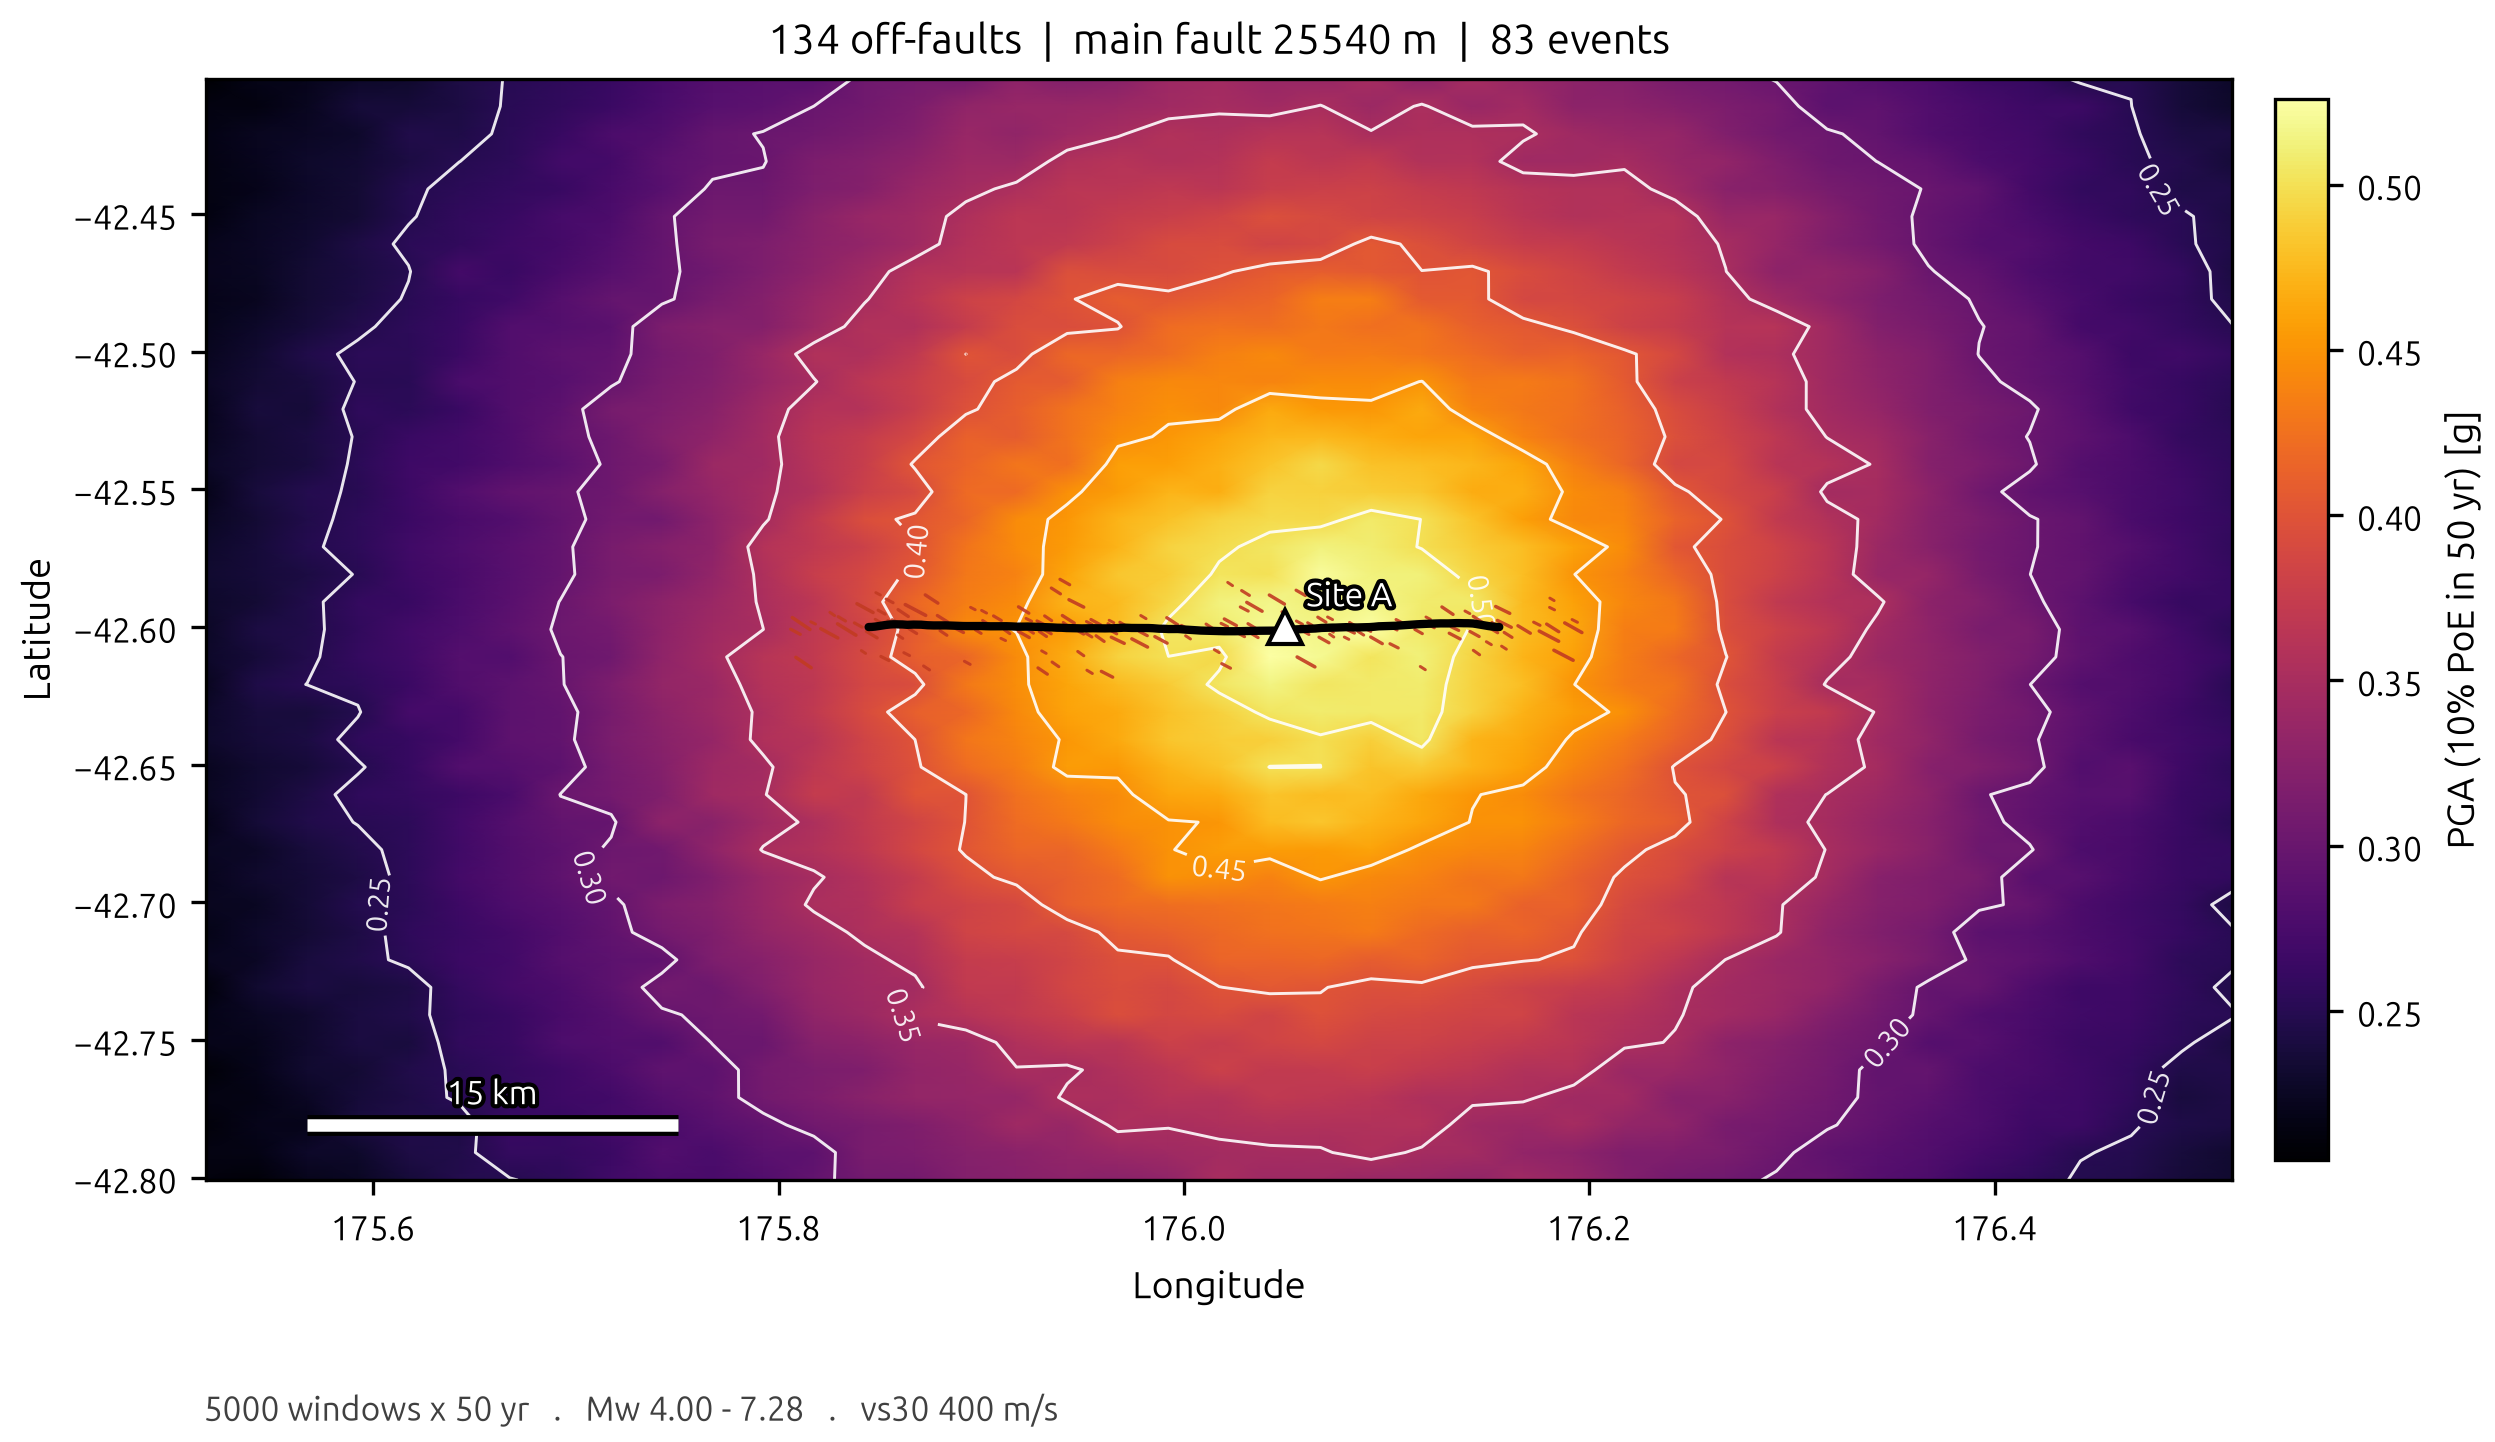
\includegraphics[width=0.95\textwidth]{./figures/hazard_mapb}
		\caption*{\scriptsize Hazard map from the synthetic catalog: PGA with 10\%
		probability of exceedance in 50 years. Main fault in black,
		subsidiary faults in red.}
		\end{figure}
	}
\end{frame}

%% ------------------------------------------------------------------
%% PART 5 - Discussion
%% ------------------------------------------------------------------

\begin{frame}[t]\frametitle{Discussion}

\textbf{What works:}
\begin{itemize}\small
  \item Geometry generator $\rightarrow$ VEGA
        $\rightarrow$ catalog $\rightarrow$ windows $\rightarrow$ GMM
        $\rightarrow$ hazard curves and maps.
  \item Magnitudes spanning $M_w \approx 4.5$--$7$ from a single
        network, with (almost) emergent Gutenberg--Richter behaviour, clustering
        and quasi-periodic large events.
\end{itemize}

\textbf{Limitations learned:}
\begin{itemize}\small
  \item Point-source distances (finite-rupture distances missing).
  \item Better constrain loading rate (tested arbitrary values).
  \item Statistical resolution is bounded by catalog length: the tail of
        the curve is limited by $\Delta / T$.
  \item Still a gap in the GR distribution ($M_w \in [3,6]$)
\end{itemize}

\textbf{Next:}

\end{frame}


%% ------------------------------------------------------------------
%% Backup
%% ------------------------------------------------------------------
\backupbegin




\backupend

\end{document}